
\section{Experiments}\label{section:eval}

\subsection{Experimental Setup}
We now use the Ultrasound Design Gallery for tuning the cascaded Laplacian pyramid diffusion.

\subsubsection{Experiment Design}
\paragraph{Sonographer Subjects}
We recruited five sonographers and a cardiologist from the Kangbuk Samsung Hospital Total Healthcare Center and asked them to optimize a video sequence of a liver images and two sequences of echocardiographic heart images.
All five sonographers are Registered Diagnostic Cardiac Sonographers (RDCS) certified by the American Registry for Diagnostic Medical Sonography (ARDMS) with at least three years of practicing experience.
The cardiologist is a actively practicing cardiologist with ten years of clinical experience.

\begin{table}
  \centering
  \caption{Hardware used for the Experiments}\label{table:specs}
  \begin{threeparttable}
  \begin{tabular}{ll}
    \toprule
    \multicolumn{1}{c}{\textbf{Type}}
    & \multicolumn{1}{c}{\textbf{Model and Specifications}}
    \\ \midrule
    Processor & Intel i7--7700HQ, 2.8 GHz (maximum 3.8 GHz) \\
    GPU       & Nvidia GeForce GTX 1050 Mobile \\
    Display   & Sharp LQ156D1, 15.6 inch, \(3840 \times 2160\), 282ppi  \\
    Memory    & 16GB DDR4--2400 \\ \bottomrule
  \end{tabular}
  \end{threeparttable}
\end{table}
%
\paragraph{Experiment Protocol}
Each of the sonographers were given access to the~\usdg~through same laptop.
The hardware specification of the laptop are shown in~\cref{table:specs}.
Then, the sonographers interact with the~\usdg~until the iteration counter indicated 15.
The first 4 iterations used random settings such that \(\vx\) is a random uniform vector and \(\vxi\) is sampled from a unit \(L_{\infty}\) hypersphere.

The sonographers were instructed to freely interact with the video control panel at any time.
However, they were strictly instructed to choose a position on the slider \textit{relative} to other positions.
Without such instruction, some users were unable to choose a candidate becase all of the positions seemed to result in equality disliked images.
Also, in some cases, all of the positions on the slider resulted in images visually indistinguisable.
For such iteration, We instructed the sonographers to choose a random position.

For evaluating the final results, we choose the parameter setting maximizing the mean utility function of each sonographer such as \( \vx^* = \argmax_{\vx} \mu\left(\vx \mid \mathcal{D}_{15} \right) \).

\subsubsection{Image Enhancement Baselines}
We evaluate the tuned cascaded Laplacian pyramid diffusion filters against a diverse range of speckle reduction algorithms.
Among diffusion algorithms, we compare against the speckle reducing anisotropic diffusion (OSRAD,~\cite{krissian_oriented_2007}), the anisotropic diffusion filter with memory based on speckle statistics (ADMSS,~\cite{ramos-llorden_anisotropic_2015}), and the multiscale nonlinear diffusion and shock filter (LPNDSF,~\cite{zhang_multiscale_2006}) methods.
Among non-local means based methods, we compare against the multiscale non-local means (MNLM,~\cite{breivik_realtime_2017}), and the non-local low-rank patch recovery (NLLR,~\cite{zhu_nonlocal_2017}) methods.
Lastly, we compare against the phase asymmetry ultrasound despeckling with fractional anisotropic diffusion and total variation (PFDTV,~\cite{mei_phase_2020}) method.


\begin{table*}
  %\vspace{-0.2in}
  \centering
\begin{threeparttable}
  \caption{Implementations and Parameter Settings of the Considered Baselines}\label{table:baselines}
\begin{tabular}{llclc}\toprule
  \multicolumn{1}{c}{\textbf{Algorithm}}          &
  \multicolumn{1}{c}{\textbf{Classification}}     &
  \multicolumn{1}{c}{\textbf{Implementation}}     &
  \multicolumn{1}{c}{\textbf{Parameter Settings}} &
  \multicolumn{1}{c}{\textbf{Reference}} \\\midrule
  OSRAD  & Diffusion       & Custom            & \(W_{\text{kuan}}= 5 \times 5\), \(c_{\text{tang}} = 0.1\), \(N_{\text{iteration}}=30\), \(\Delta t = 1\) & \cite{krissian_oriented_2007}  \\
  ADMSS  & Diffusion       & Official\tnote{1} & \(N_{\text{class}} = 4\), \(N_{\text{memory}}=5\), \(N_{\text{iteration}} = 20\), \(\sigma = 0.1\), \(\rho = 0.1\)  & \cite{ramos-llorden_anisotropic_2015} \\
  LPNDSF & Diffusion       & Custom            & \(r = [0.1, 1.0, 0.1]\), \(k = [0.3, 0.1, 0.1]\) & \cite{zhang_multiscale_2006} \\
  MNLM   & Non-local mean  & Custom            & \(M = 19 \times 19\), \(K = 3 \times 3\), \(I = 5\), \(h=0.1\) & \cite{breivik_realtime_2017} \\
  NLLR   & Non-local mean \& Low-rank recon.   & Official\tnote{2} & \(H = 10\), \(\beta = 10\) & \cite{zhu_nonlocal_2017} \\
  PFDTV  & Diffusion \& TV regularization    & Custom\tnote{3}   & \(N_{\text{iteration}} = 10\), \(s=15\) & \cite{mei_phase_2020} \\
  \bottomrule
\end{tabular}
\begin{tablenotes}
  \item[1] \url{https://www.mathworks.com/matlabcentral/fileexchange/52988-anisotropic-diffusion-with-memory-based-on-speckle-statistics-for-ultrasound-images}
  \item[2] \url{https://appsrv.cse.cuhk.edu.hk/~lzhu/webpage_despeckling_cvpr2017/index.html}
  \item[3] Based on the official implementation available at \url{https://github.com/Binjie-Qin/PFDTV}.
\end{tablenotes}
\end{threeparttable}
\vspace{-0.1in}
\end{table*}

%%% Local Variables:
%%% TeX-master: "master"
%%% End:

%
\subsubsection{Implementations and Tuning of the Baselines}
To ensure a fair comparison, we will use the official implementation of the considered baselines whenever available.
The implementations and parameter settings of the considered baselines are organized in~\cref{table:baselines}.
For the OSRAD, MNLM, LPNDSF, and PFDTV algorithms, we reimplemented the algorithms according to the descriptions in the original papers.
While the official implementation of PFDTV is publically available online, we had to reimplement it due to numerical issues.

\paragraph{Issues with Pixel Spacing}
For the NLLR and PFDTV, the pixel spacing of the data used in the original works (\(300 \times 225\)) differed significantly with ours (our images are \(800 \times 600\)).
Because of this, when applied to our data, the results were qualitatively different from those reported in the original papers.
Thus, for PFDTV and NLLR, we downscaled the images by \(40\%\), applyed the respective methods, and then upscaled the images for evaluation.

\paragraph{Input Transformations}
While often not clearly stated, the input format of ultrasound speckle reduction methods vary.
For example, OSRAD requires the input image to be in natural scale rather than logarithmic scale.
Therefore, for OSRAD, we decompressed the log-compressed images as recommended by~\cite{yongjianyu_generalized_2004} and then recompressed the output.
Other than OSRAD, we applied all methods to log-compressed images with pixel intensities in the range of \([0, 255]\).

\subsubsection{Metrics}
For objective quality assessment, we apply the following quality metrics to the image \textit{before} dynamic range adjustment.
All results are presented up to three significant digits.

\paragraph{(Speckle) Signal-to-Noise Ratio (SNR)}
The SNR measures the amount of speckle noise relative to the mean response of a region-of-interest.
It is given as
\begin{align}
  \mathrm{SSNR} \texttt{[dB]} = 10 \log_{10} \frac{\mu}{\sigma}
\end{align}
where \(\mu\) is the mean response and \(\sigma\) is the standard deiviation of the region-of-interest.
When computed against a fully-formed speckle region, the SNR is called the \textit{speckle} SNR (SSNR).
In this case, \(\sigma\) corresponds to the noise standard deiviation.
We present the SNR in decibel scale.

\paragraph{Contrast-to-Noise Ratio (CNR)}
The CNR first introduced by Patterson and Foster~\cite{patterson_improvement_1983} measures the mean response difference of two regions-of-interests relative to their standard deviations such as
\begin{align}
  \mathrm{CNR} \texttt{[dB]} = 10 \log_{10} \frac{| \mu_{1} - \mu_{2} |}{ \sqrt{\sigma^2_1 + \sigma^2_2} }
\end{align}
where \(\mu_1, \mu_2\) are the mean responses of the regions-of-interests, and \(\sigma_1, \sigma_2\) are their standard deviations, respectively.
While the CNR has been shown to be loosely related to the detectibility of lesions~\cite{smith_ultrasound_1984}, Rindal \textit{et al.} has shown that it can be misleading when used against methods altering the natural dynamic range~\cite{rindal_effect_2019}.
Also, the CNR can be viewed as a special case of the Q-index used in~\cite{tay_ultrasound_2006} where only two classes are used.
We present the CNR in decibel scale.

%% Nonetheless, the CNR still provides a measure of relative contrast.

\paragraph{Generalized CNR (gCNR)}
As a remedy to the limitations of the CNR, Rodriguez-Molares \textit{et al.}~\cite{rodriguez-molares_generalized_2020} proposed the gCNR metric.
They also showed that the gCNR is less affected by dynamic range alternations, making it a better general performance metric for medical utlrasound.
The gCNR is defined as
\begin{align}
  \text{gCNR} = 1 - \int_{-\infty}^{\infty} \min\big(p_1\left(x\right), p_2\left(x\right)\big) \, dx
\end{align}
where \(p_1\left(x\right)\) and \(p_2\left(x\right)\) are the probability densities of \(x\) subject to the pixel intensity distributions of the regions-of-interests 1 and 2.
It is apparent from the explicit use of probabilities that the gCNR is directly related to the detection probability of lesions.

\paragraph{Structural Similarity Index (SSIM)}
The SSIM is a metric for measuring the \textit{structural} similarity of images, which is derived as a product of the differences in lumiance, structure, and contrast~\cite{wang_image_2004a}.
Wang \textit{et al.} has shown that the SSIM is aligned with the perception of humans, and is sensitive to distortions such as blur and blockiness.
Mathematically, the SSIM between image 1 and 2 is computed such that
\begin{align}
  \mathrm{SSIM} = \frac{1}{N} \sum_k^N \frac{
    (2 \mu_{1,k} \, \mu_{2, k} + C_1)(2 \sigma_{12, k} + C_2)
  }{
    (\mu_{1,k}^2 + \mu_{2,k}^2 + C_1) ( \sigma_{1,k}^2 + \sigma_{2,k}^2 + C_2)
  }
\end{align}
where \(\mu_{1,k}\), \(\mu_{2,k}\), are the mean of the \(k\)th patch on each images, \(\sigma_{1,k}^2\), \(\sigma_{2,k}^2\) are their respective variances, and \(\sigma_{12, k}\) is the covariance of the two.
The SSIM is taken as an average over all the patches, which are taken by a \(11 \times 11\) Gaussian window of standard deviation 1.5.
The coefficients are chosen as \(C_1 = 1 \times 10^{-4}, C_2 = 9 \times 10^{-4} \).
We use the implementation of the \texttt{ImageQualityIndexes.jl} library\footnote{\url{https://github.com/JuliaImages/ImageQualityIndexes.jl}}

\paragraph{\(S_3\) Index}
Finally, we use a metric for evaluating the blurriness of the images.
Blurriness metrics have not been tradiionally used for evaluating the quality of medical ultrasound images.
However, we will later show that blurriness is an important quality factor for sonographers.
In this work, we use the \(S_3\) metric proposed in~\cite{vu_bf_2012}.
The \(S_3\) value of the \(k\)th patch is defined as a harmonic mean such that
\begin{align}
  S_3\left(k\right) = \sqrt{S_1\left(k\right)} \sqrt{S_2\left(k\right)}
\end{align}
where \(S_1\left(k\right)\) and \(S_2\left(k\right)\) are its spatial and spectral measures of sharpness.
The final \(S_3\) index of an image is given as the average of the top 1\% \(S_3\) values.
We use the official implementation\footnote{\url{https://sites.google.com/site/cuongvt101/research/Sharpness-measure}} provided by the authors.

%
\begin{figure}[h]
  \centering
  \subfloat[Liver image]{
    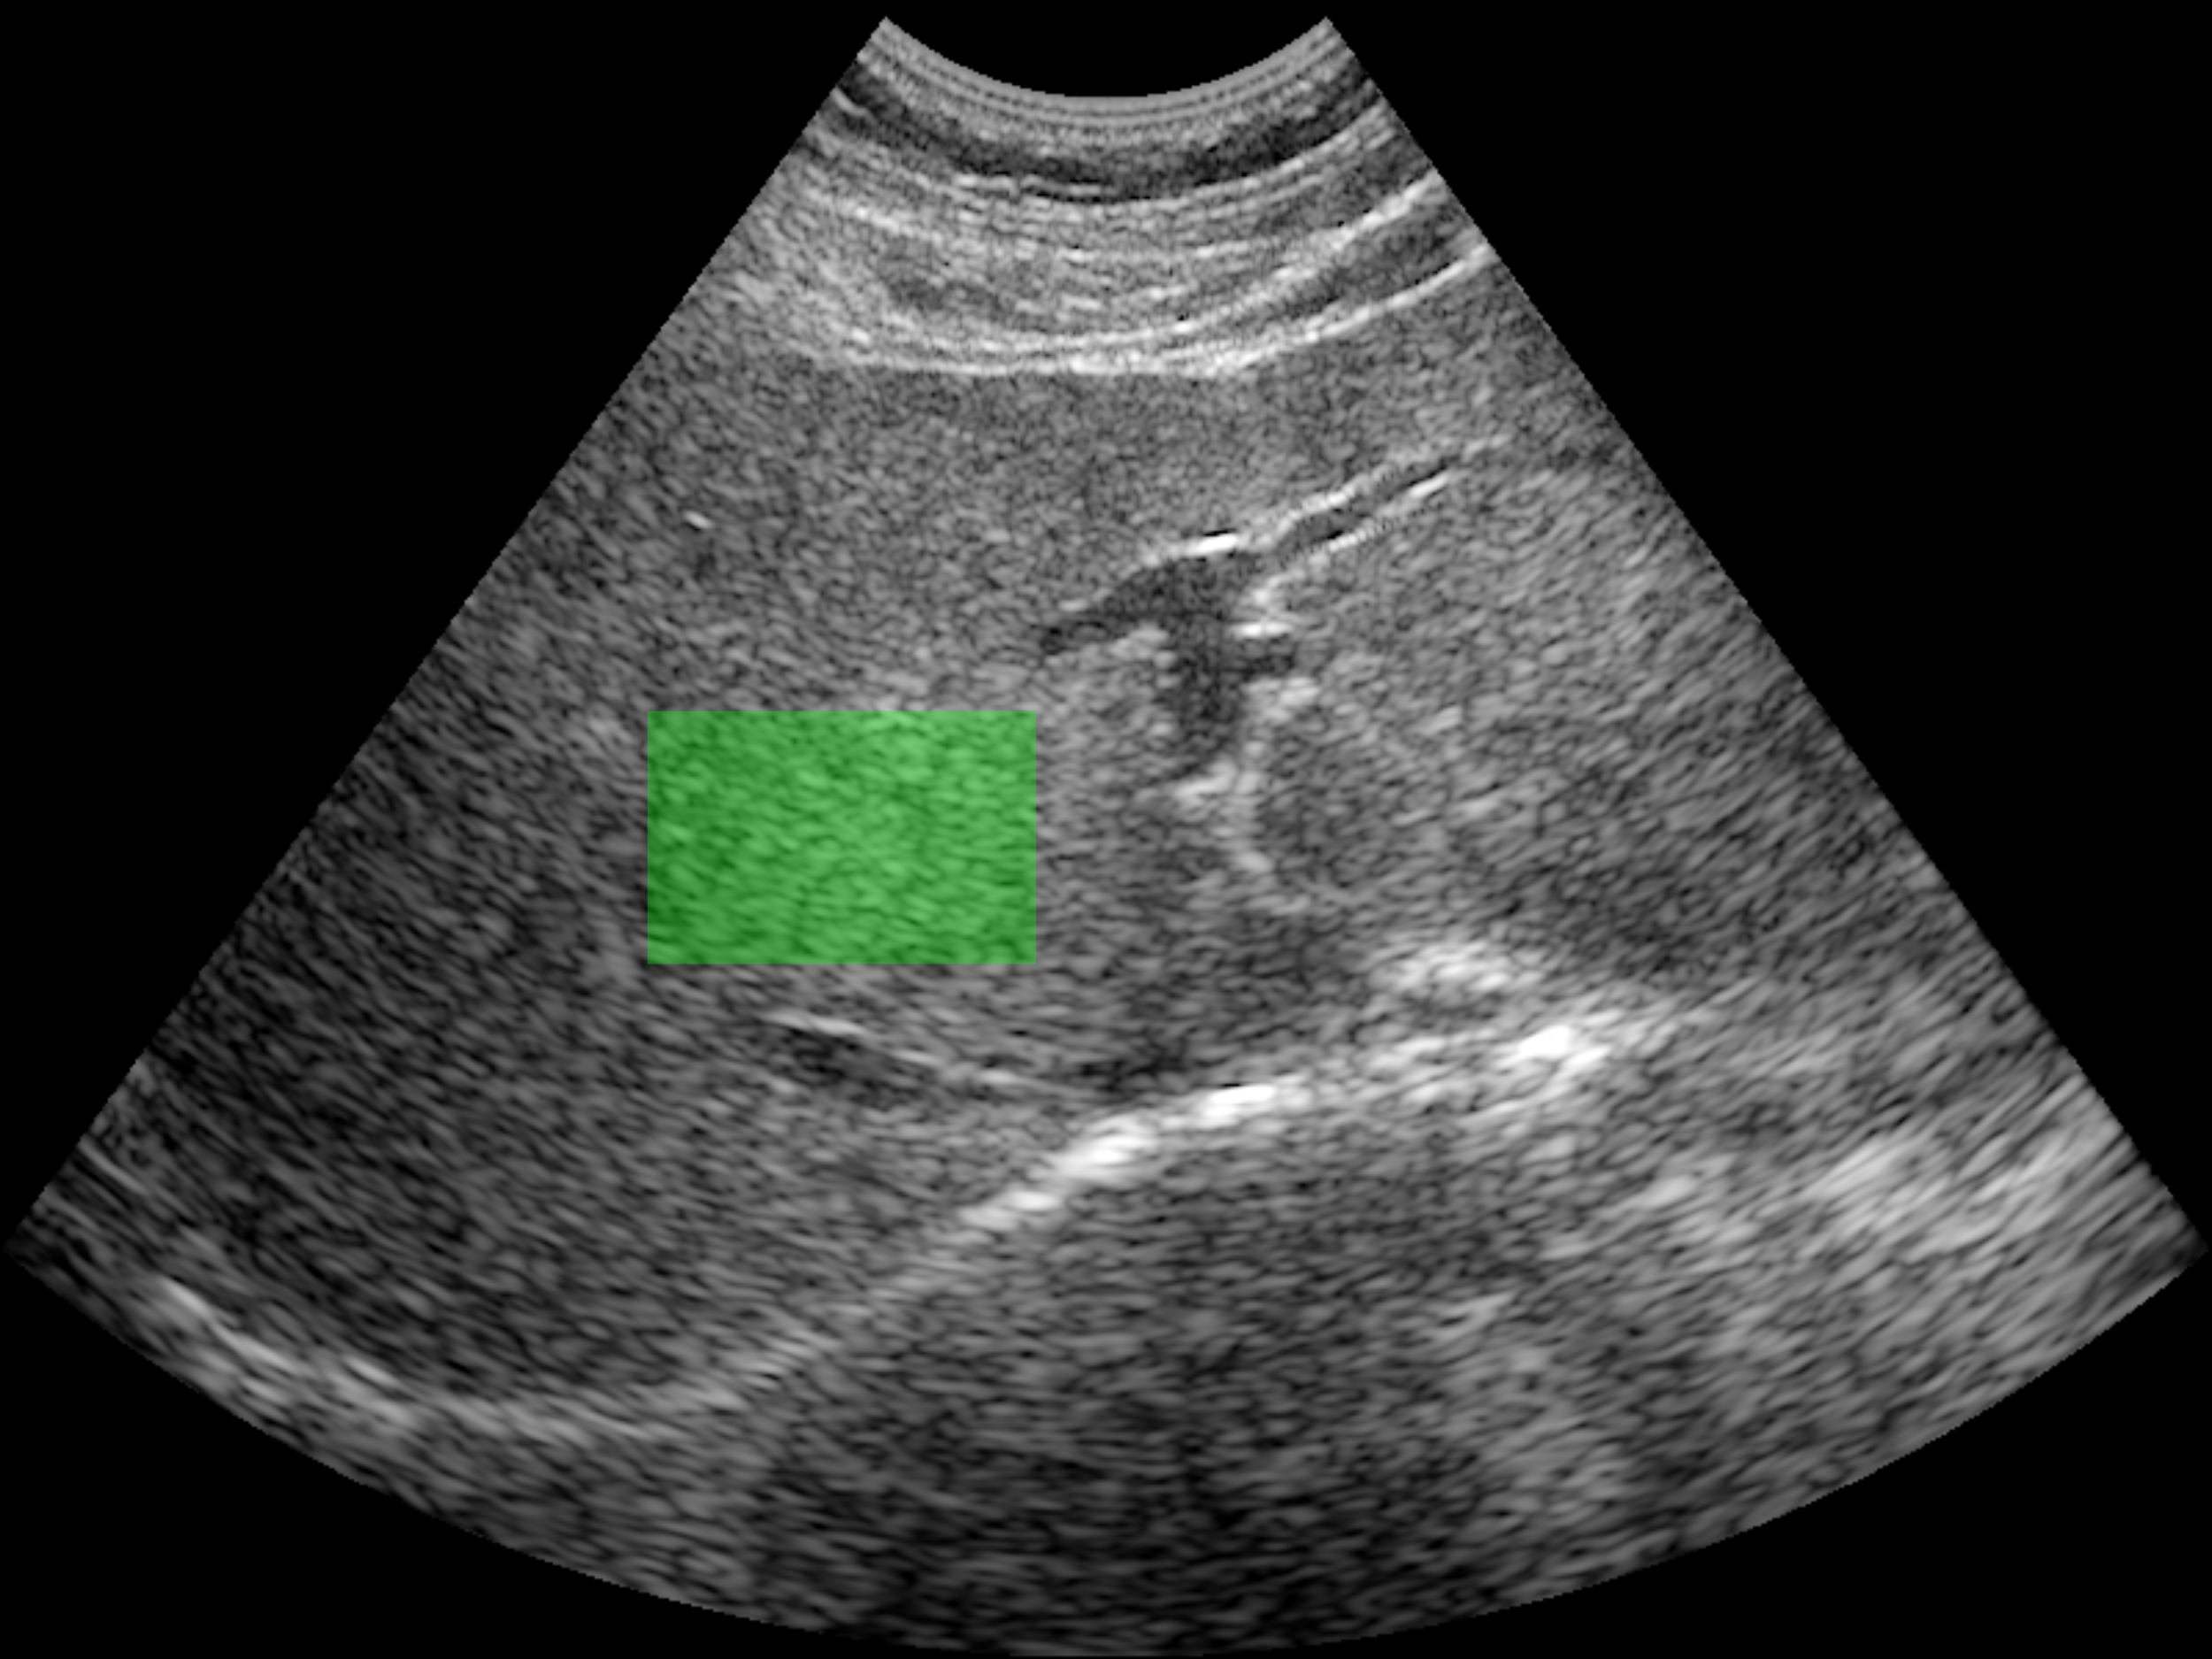
\includegraphics[height=3cm]{figures/liver_roi.png}\label{fig:liver_roi}
  }
  \subfloat[Cardiac image]{
    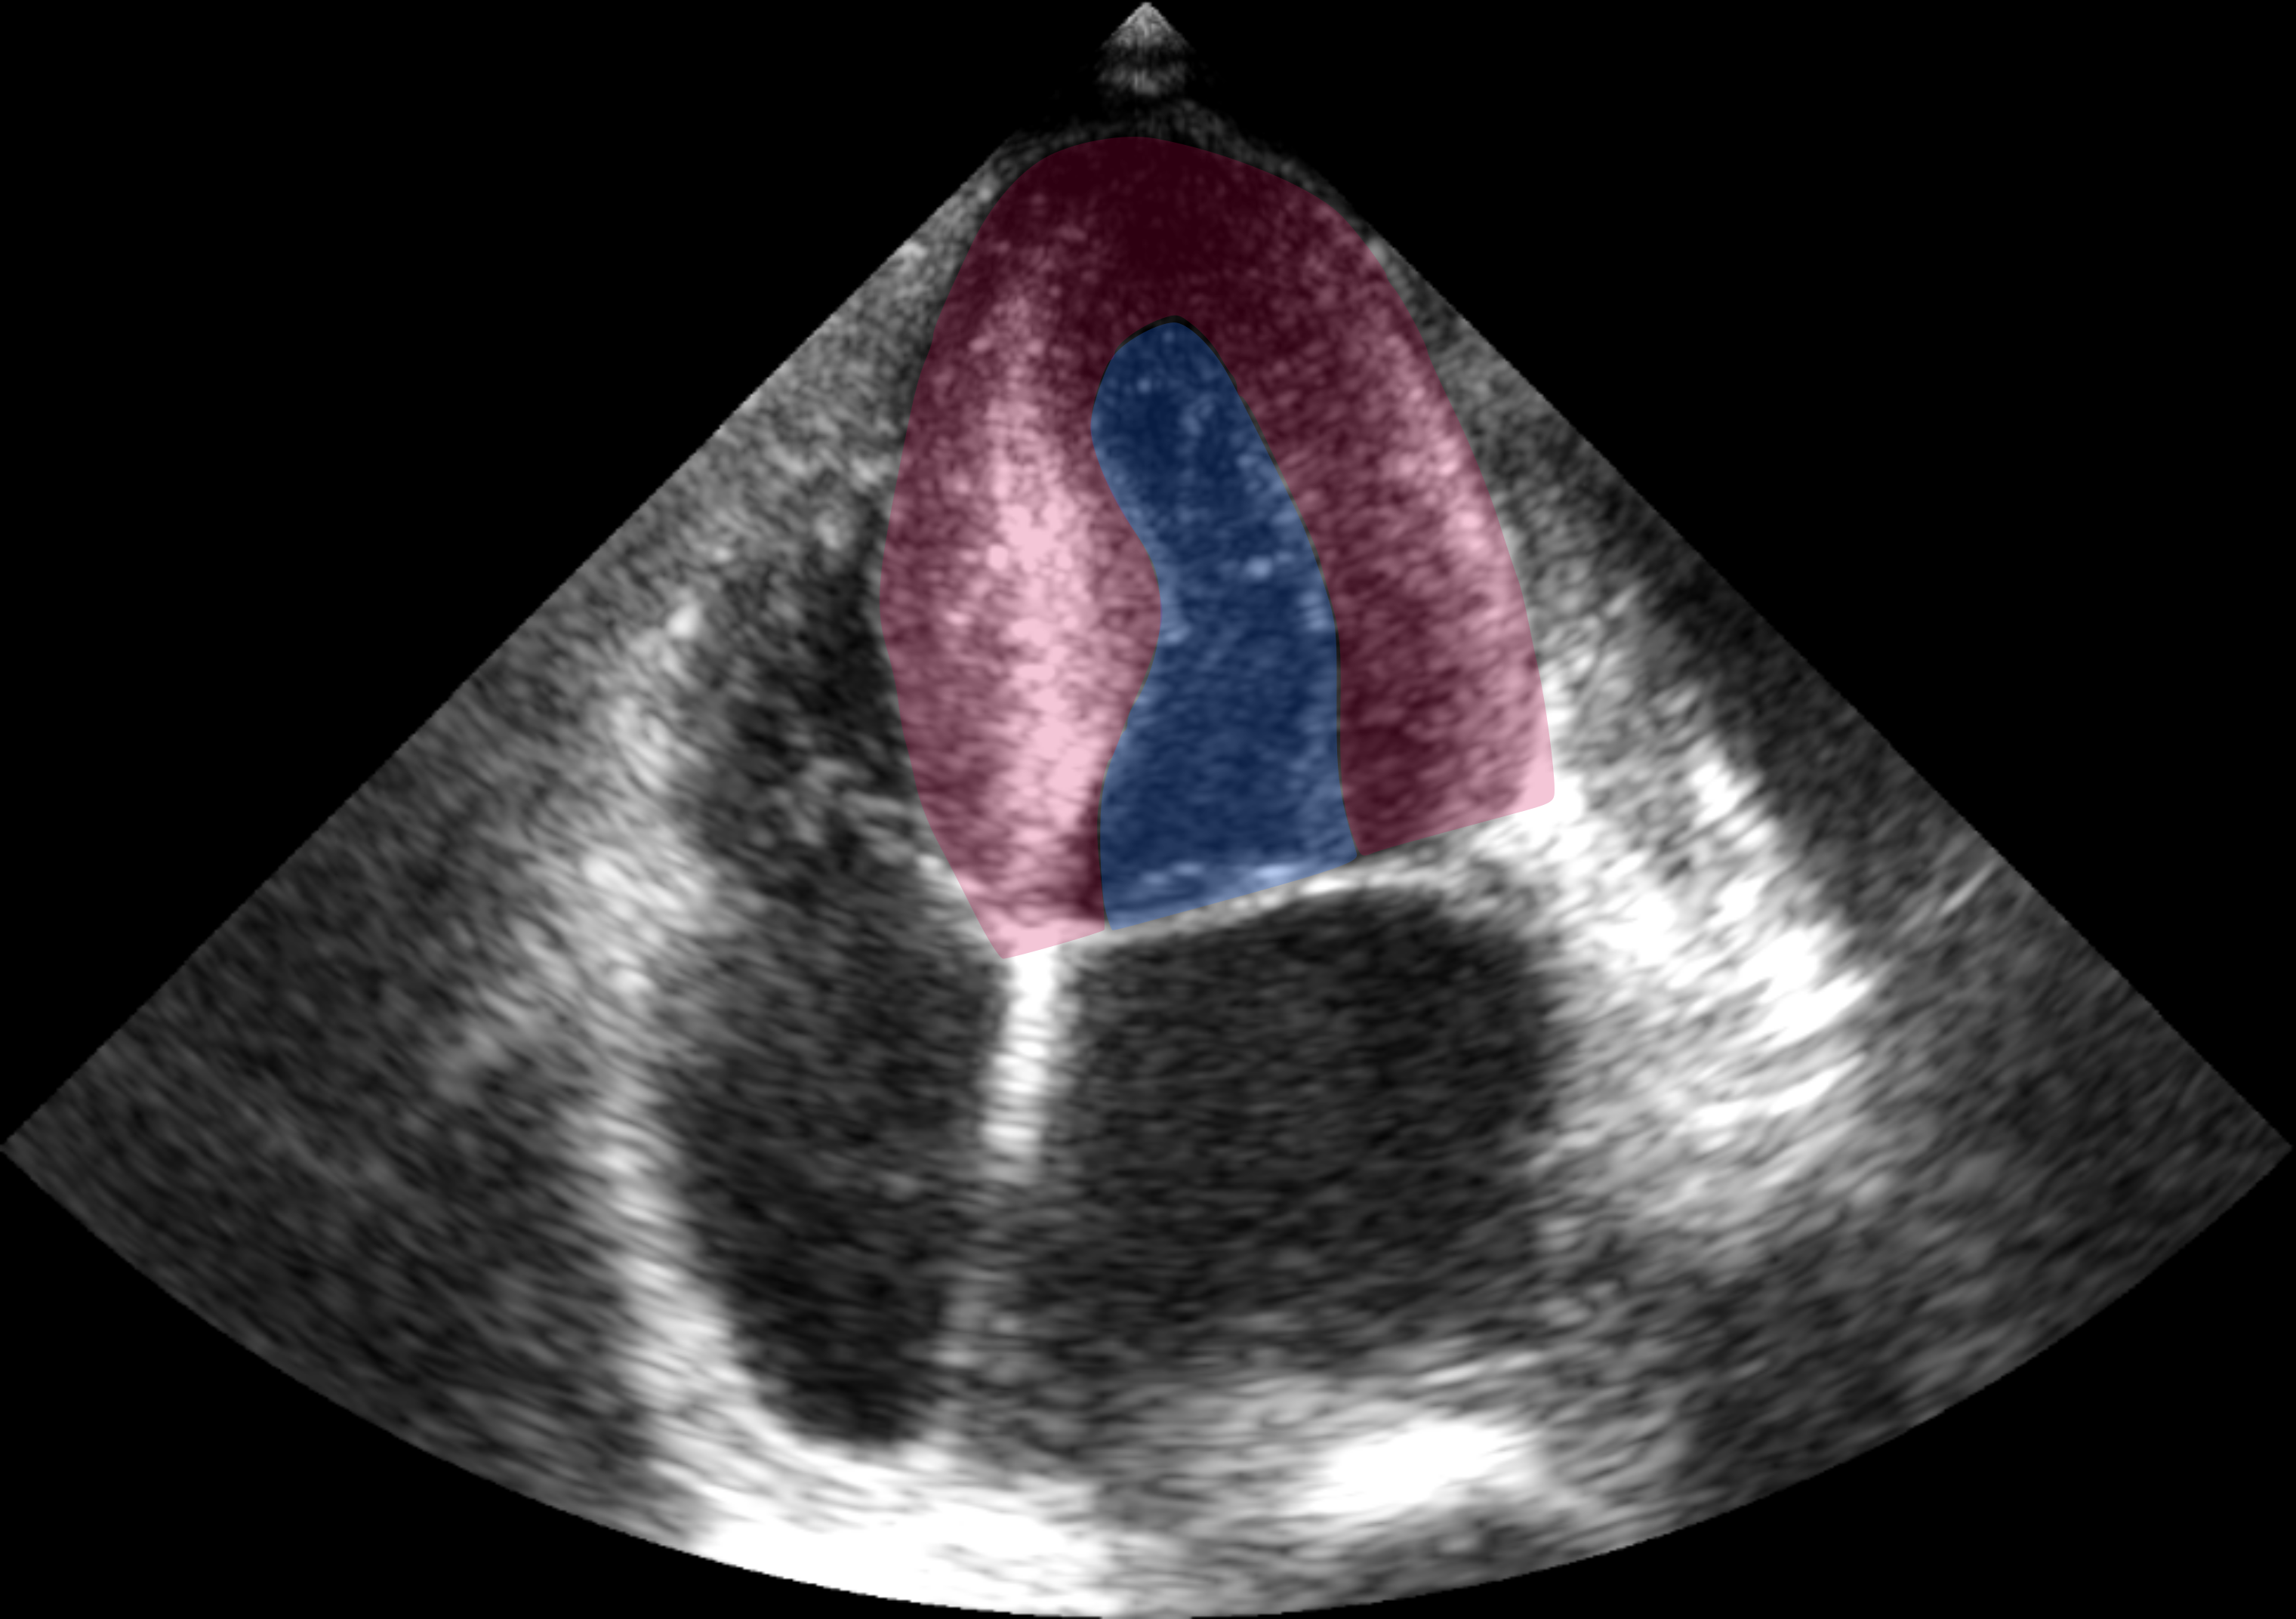
\includegraphics[height=3cm]{figures/cardiac_roi.png}\label{fig:cardiac_roi}
  }
  \caption{Regions-of-interests used for using the objective performance metrics.
    (a) The \textcolor{orange}{orange} region is used for computing the SSNR.
    (b) The \textcolor{red}{red} region (endocardium of the left ventricle) and \textcolor{blue}{blue} region (blood of the left ventricle) are used for computing the gCNR and CNR.
    The red region is also used for computing the SNR.
  }\label{fig:roi}
\end{figure}
% 
\paragraph{Regions-of-Interests}
The regions-of-interests used for computing the performance metrics are shown in~\cref{fig:roi}.
For the liver image, we compute the metrics over multiple frames, while for the echocardiographic image, we compute the metrics only using the presented frame.


\begin{figure*}
  \centering
  \begin{subfigure}[b]{0.15\textwidth}
    \begin{tikzpicture}[
        spy using outlines={%
          rectangle,magnification=3,size=\textwidth,
          every spy on node/.append style={transparentwindow}
        }
      ]
      \node (figA) at (0.0,0.0) {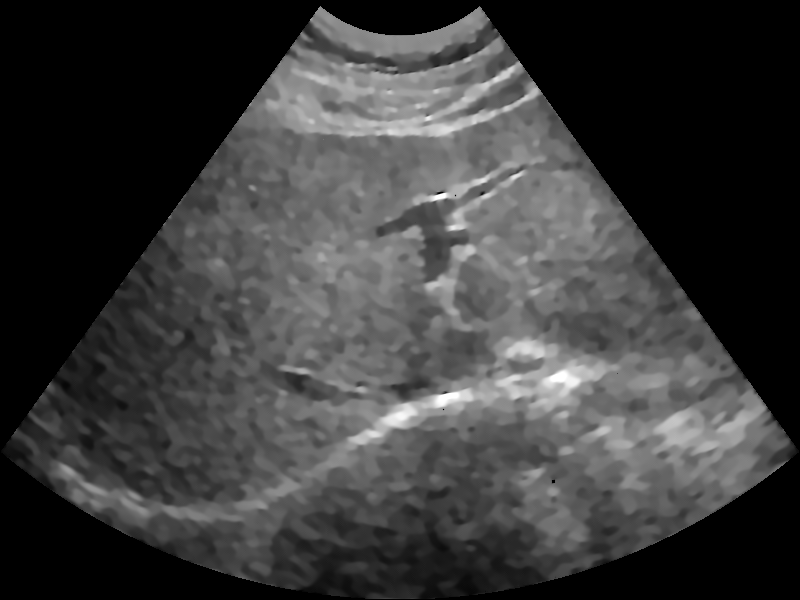
\includegraphics[width=\textwidth, trim={4cm 4cm 4cm 0cm}, clip]{figures/liver1_osrad.png}};
      \spy on (0.15, 0.0) in node [redwindow, anchor=north] at ($(figA.south)$);
    \end{tikzpicture}
    \caption{OSRAD}\label{fig:liver1_osrad}
  \end{subfigure}%
  \begin{subfigure}[b]{0.15\textwidth}
    \begin{tikzpicture}[
        spy using outlines={%
          rectangle, magnification=3,size=\textwidth,
          every spy on node/.append style={transparentwindow}
        }
      ]
      \node (figA) at (0.0,0.0) {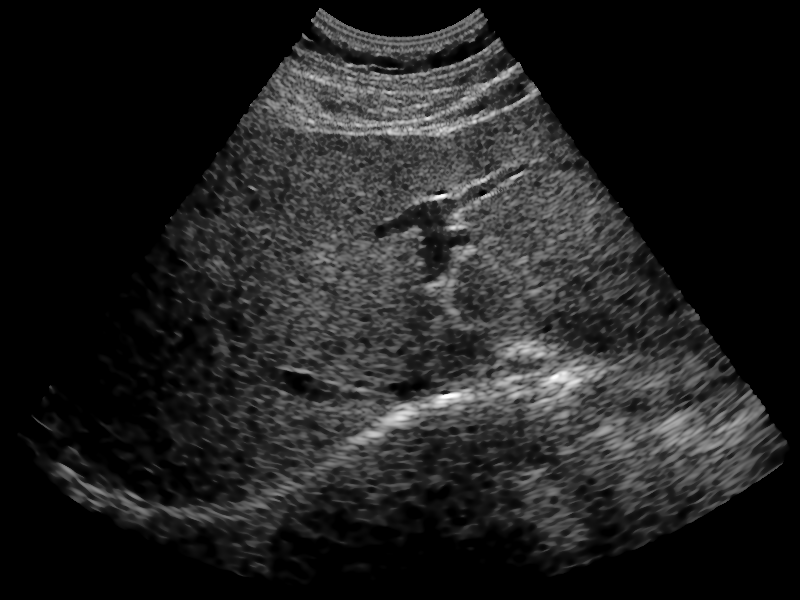
\includegraphics[width=\textwidth, trim={4cm 4cm 4cm 0cm}, clip]{figures/liver1_admss.png}};
      \spy on (0.15, 0.0) in node [redwindow, anchor=north] at ($(figA.south)$);
    \end{tikzpicture}
    \caption{ADMSS}\label{fig:liver1_admss}
  \end{subfigure}%
  \begin{subfigure}[b]{0.15\textwidth}
    \begin{tikzpicture}[
        spy using outlines={%
          rectangle, magnification=3,size=\textwidth,
          every spy on node/.append style={transparentwindow}
        }
      ]
      \node (figA) at (0.0,0.0) {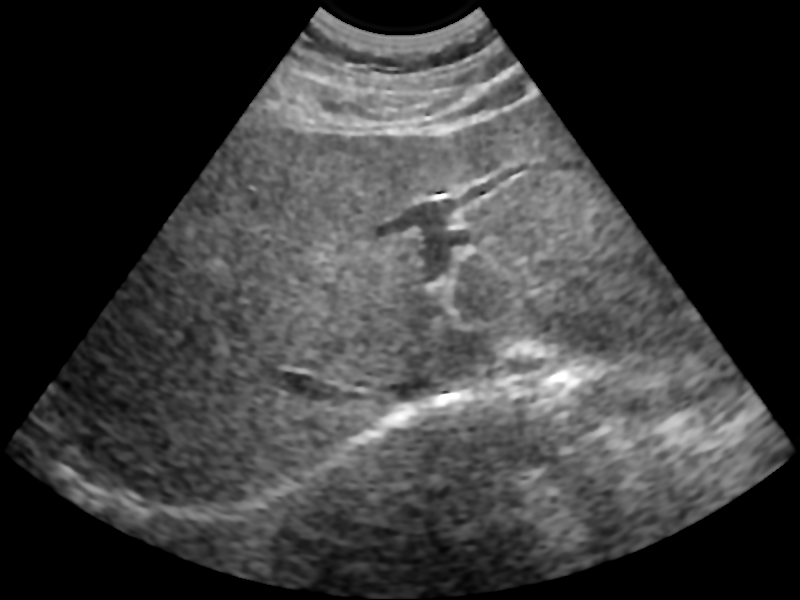
\includegraphics[width=\textwidth, trim={4cm 4cm 4cm 0cm}, clip]{figures/liver1_lpndsf.png}};
      \spy on (0.15, 0.0) in node [redwindow, anchor=north] at ($(figA.south)$);
    \end{tikzpicture}
    \caption{LPNDSF}\label{fig:liver1_lpndsf}
  \end{subfigure}%
  \begin{subfigure}[b]{0.15\textwidth}
    \begin{tikzpicture}[
        spy using outlines={%
          rectangle,magnification=3,size=\textwidth,
          every spy on node/.append style={transparentwindow}
        }
      ]
      \node (figA) at (0.0,0.0) {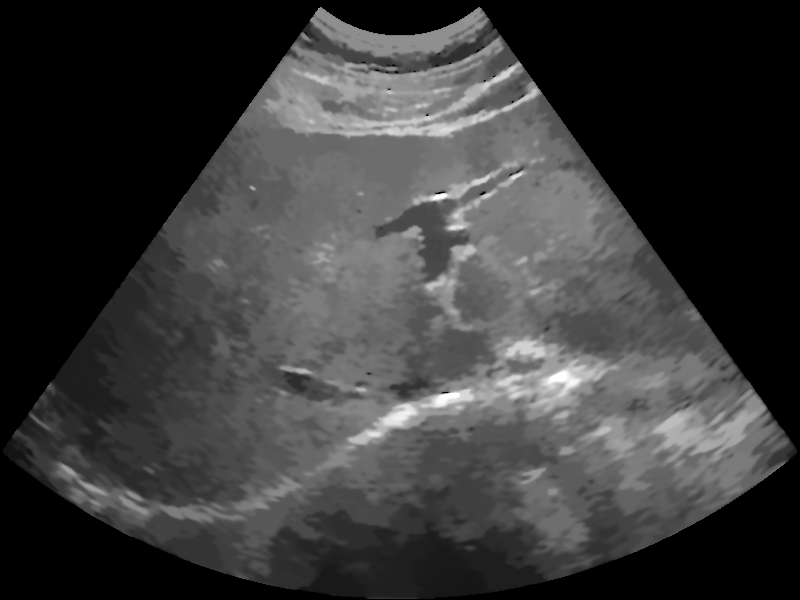
\includegraphics[width=\textwidth, trim={4cm 4cm 4cm 0cm}, clip]{figures/liver1_mnlm.png}};
      \spy on (0.15, 0.0) in node [redwindow, anchor=north] at ($(figA.south)$);
    \end{tikzpicture}
    \caption{MNLM}\label{fig:liver1_mnlm}
  \end{subfigure}%
  \begin{subfigure}[b]{0.15\textwidth}
    \begin{tikzpicture}[
        spy using outlines={%
          rectangle,magnification=3,size=\textwidth,
          every spy on node/.append style={transparentwindow}
        }
      ]
      \node (figA) at (0.0,0.0) {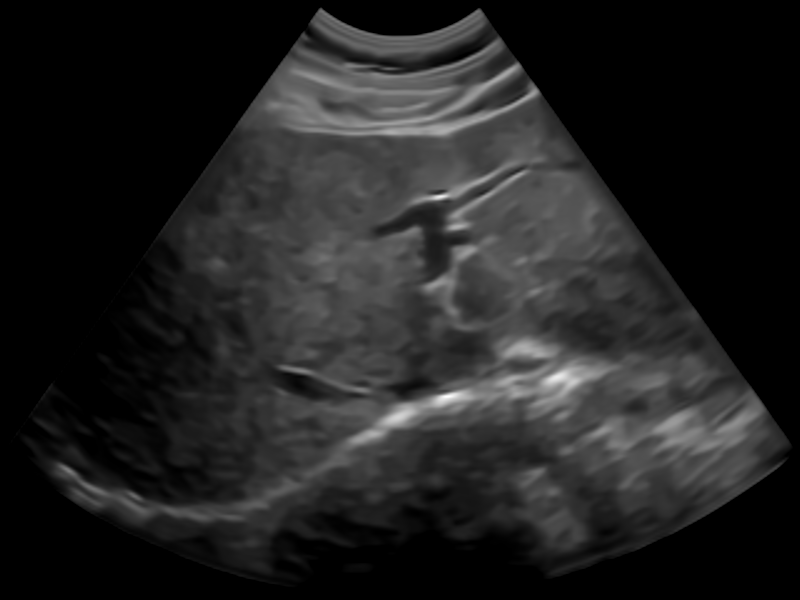
\includegraphics[width=\textwidth, trim={4cm 4cm 4cm 0cm}, clip]{figures/liver1_nllr.png}};
      \spy on (0.15, 0.0) in node [redwindow, anchor=north] at ($(figA.south)$);
    \end{tikzpicture}
    \caption{NLLR}\label{fig:liver1_nllr}
  \end{subfigure}%
  \begin{subfigure}[b]{0.15\textwidth}
    \begin{tikzpicture}[
        spy using outlines={%
          rectangle,magnification=3,size=\textwidth,
          every spy on node/.append style={transparentwindow}
        }
      ]
      \node (figA) at (0.0,0.0) {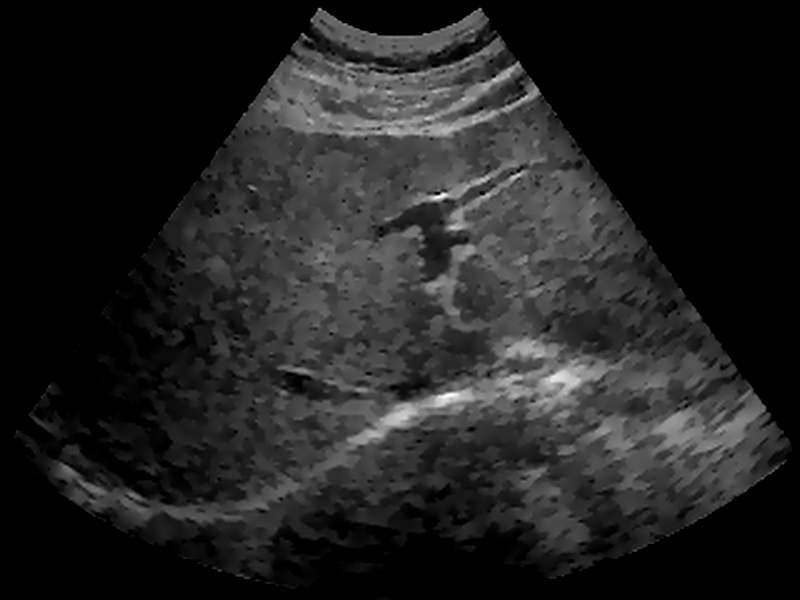
\includegraphics[width=\textwidth, trim={4cm 4cm 4cm 0cm}, clip]{figures/liver1_pfdtv.png}};
      \spy on (0.15, 0.0) in node [redwindow, anchor=north] at ($(figA.south)$);
    \end{tikzpicture}
    \caption{PFDTV}\label{fig:liver1_pfdtv}
  \end{subfigure}\\
  \begin{subfigure}[b]{0.15\textwidth}
    \begin{tikzpicture}[
        spy using outlines={%
          rectangle,magnification=3,size=\textwidth,
          every spy on node/.append style={transparentwindow}
        }
      ]
      \node (figA) at (0.0,0.0) {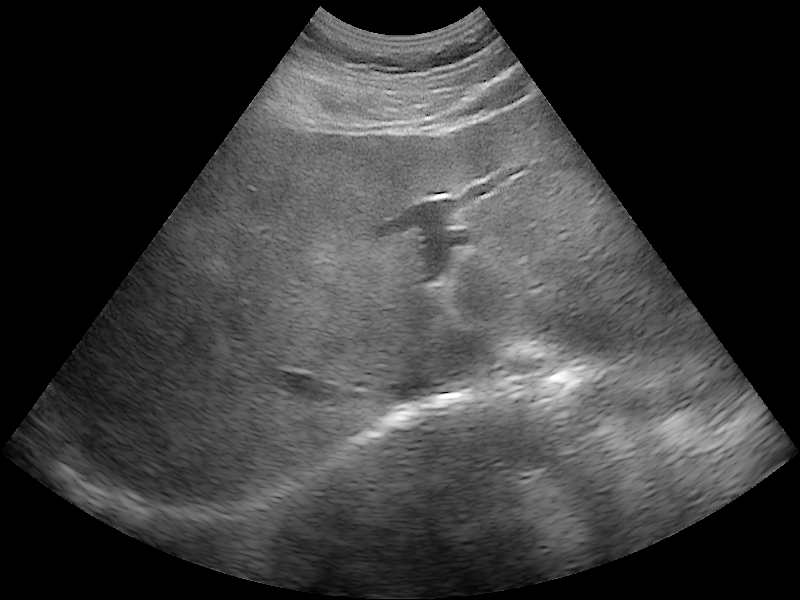
\includegraphics[width=\textwidth, trim={4cm 4cm 4cm 0cm}, clip]{figures/liver1_clpdQ.png}};
      \spy on (0.15, 0.0) in node [redwindow, anchor=north] at ($(figA.south)$);
    \end{tikzpicture}
    \caption{CLPD-SSNR}\label{fig:liver1_clpdssnr}
  \end{subfigure}%
  \begin{subfigure}[b]{0.15\textwidth}
    \begin{tikzpicture}[
        spy using outlines={%
          rectangle,magnification=3,size=\textwidth,
          every spy on node/.append style={transparentwindow}
        }
      ]
      \node (figA) at (0.0,0.0) {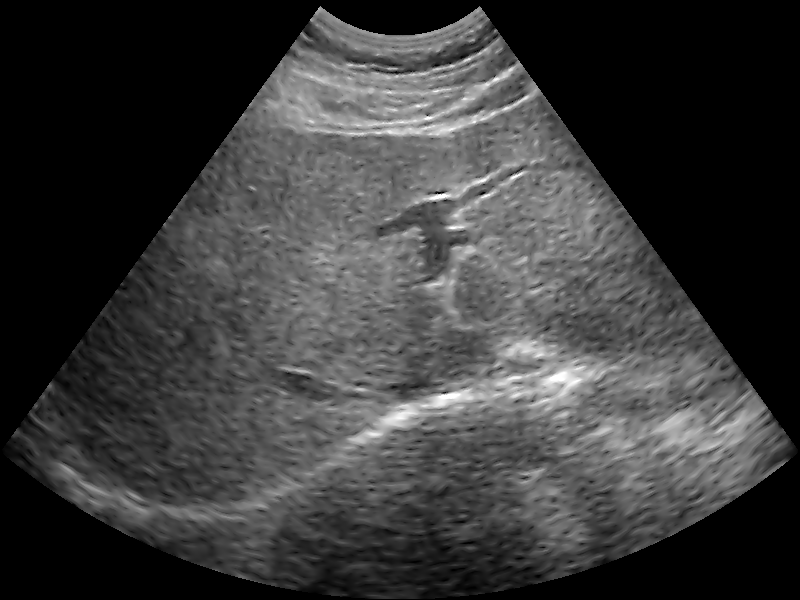
\includegraphics[width=\textwidth, trim={4cm 4cm 4cm 0cm}, clip]{figures/liver1_clpda.png}};
      \spy on (0.15, 0.0) in node [redwindow, anchor=north] at ($(figA.south)$);
    \end{tikzpicture}
    \caption{CLPD-A}\label{fig:liver1_clpda}
  \end{subfigure}%
  \begin{subfigure}[b]{0.15\textwidth}
    \begin{tikzpicture}[
        spy using outlines={%
          rectangle,magnification=3,size=\textwidth,
          every spy on node/.append style={transparentwindow}
        }
      ]
      \node (figA) at (0.0,0.0) {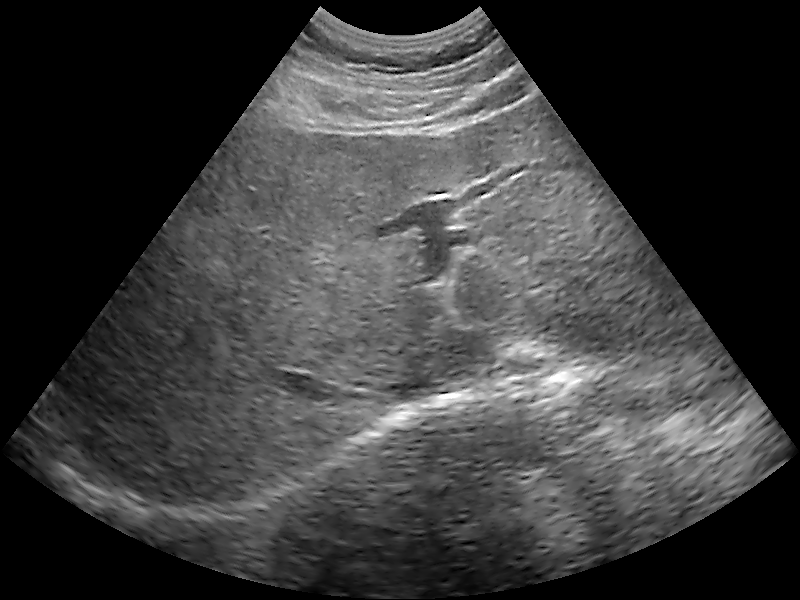
\includegraphics[width=\textwidth, trim={4cm 4cm 4cm 0cm}, clip]{figures/liver1_clpdb.png}};
      \spy on (0.15, 0.0) in node [redwindow, anchor=north] at ($(figA.south)$);
    \end{tikzpicture}
    \caption{CLPD-B}\label{fig:liver1_clpdb}
  \end{subfigure}%
  \begin{subfigure}[b]{0.15\textwidth}
    \begin{tikzpicture}[
        spy using outlines={%
          rectangle,magnification=3,size=\textwidth,
          every spy on node/.append style={transparentwindow}
        }
      ]
      \node (figA) at (0.0,0.0) {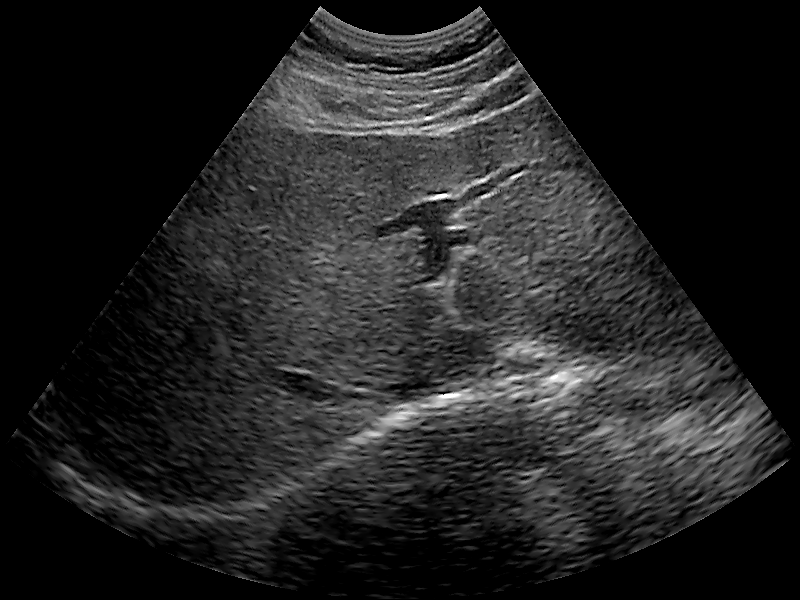
\includegraphics[width=\textwidth, trim={4cm 4cm 4cm 0cm}, clip]{figures/liver1_clpdc.png}};
      \spy on (0.15, 0.0) in node [redwindow, anchor=north] at ($(figA.south)$);
    \end{tikzpicture}
    \caption{CLPD-C}\label{fig:liver1_clpdc}
  \end{subfigure}%
  \begin{subfigure}[b]{0.15\textwidth}
    \begin{tikzpicture}[
        spy using outlines={%
          rectangle,magnification=3,size=\textwidth,
          every spy on node/.append style={transparentwindow}
        }
      ]
      \node (figA) at (0.0,0.0) {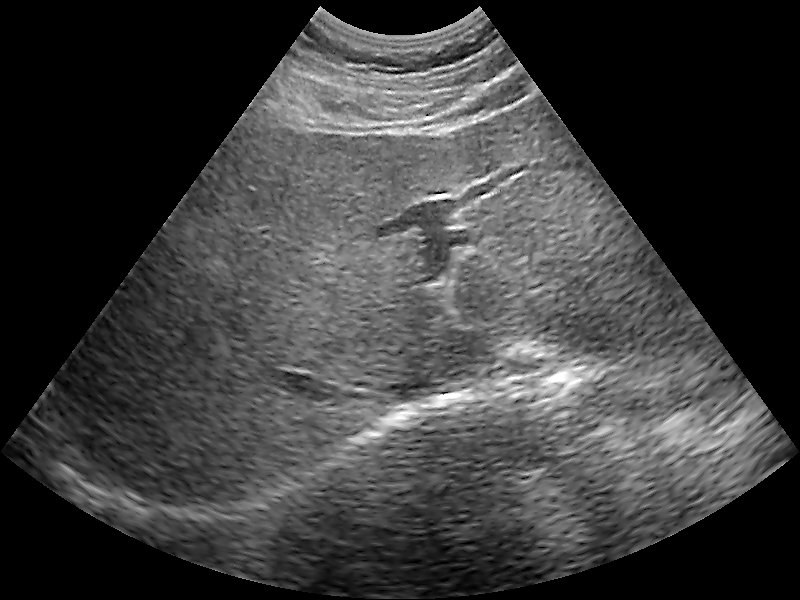
\includegraphics[width=\textwidth, trim={4cm 4cm 4cm 0cm}, clip]{figures/liver1_clpdd.png}};
      \spy on (0.15, 0.0) in node [redwindow, anchor=north] at ($(figA.south)$);
    \end{tikzpicture}
    \caption{CLPD-D}\label{fig:liver1_clpdd}
  \end{subfigure}%
  \begin{subfigure}[b]{0.15\textwidth}
    \begin{tikzpicture}[
        spy using outlines={%
          rectangle,magnification=3,size=\textwidth,
          every spy on node/.append style={redwindow}
        }
      ]
      \node (figA) at (0.0,0.0) {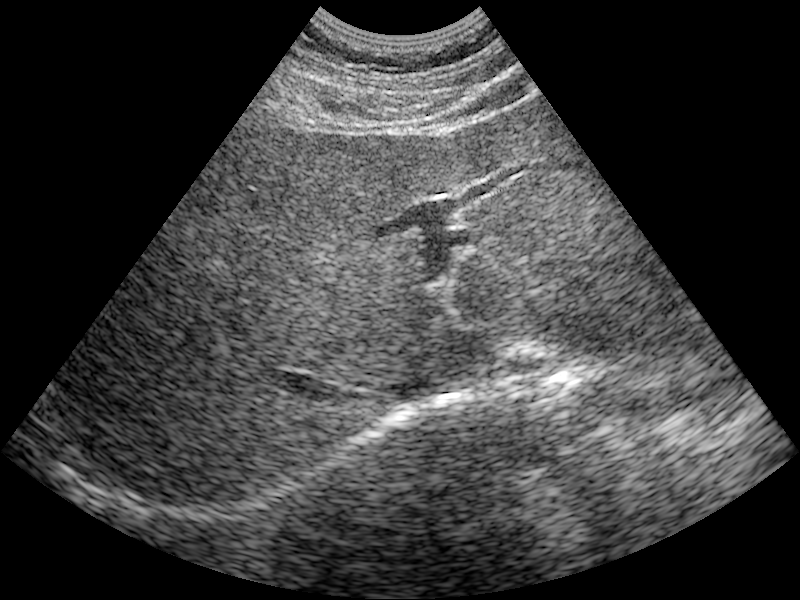
\includegraphics[width=\textwidth, trim={4cm 4cm 4cm 0cm}, clip]{figures/liver1.png}};
      \spy on (0.15, 0.0) in node [redwindow, anchor=north] at ($(figA.south)$);
    \end{tikzpicture}
    \caption{Original}\label{fig:liver_original}
  \end{subfigure}
  \caption{Results on a liver subcostal-view image.}\label{fig:liver1}
\end{figure*}

%%% Local Variables:
%%% TeX-master: "master"
%%% End:

%
\begin{table*}
  \centering
  \caption{Objective Performance Comparison on a Liver}\label{table:liver1}
  \begin{threeparttable}
  \begin{tabular}{llrrr}
    \toprule
    & \multicolumn{1}{c}{\textbf{Algorithm}}
    & \multicolumn{1}{c}{\textbf{SSNR} \texttt{[dB]}}
    & \multicolumn{1}{c}{\textbf{SSIM}}
    & \multicolumn{1}{c}{\(\mathbf{S_{3}}\)} \\\midrule
    \multirow{6}{*}{Baselines} & OSRAD & \textbf{20.8 (20.3, 21.2)} & 0.792 (0.791, 0.794) & 0.476 (0.473, 0.481)\\
    & ADMSS & 16.9 (16.5, 17.4) & \textbf{0.927 (0.893, 0.963)} & 0.350 (0.347, 0.353) \\
    & LPNDSF & 19.7 (19.4, 20.0) & 0.763 (0.762, 0.764)         & 0.343 (0.340, 0.346) \\
    & MNLM & \textbf{22.1 (21.6, 22.7)} & 0.811 (0.809, 0.812)  & 0.033 (0.329, 0.342) \\
    & NLLR & \textbf{22.0 (21.6, 22.5)} & 0.764 (0.762, 0.765)  & 0.141 (0.140, 0.142) \\
    & PFDTV & \textbf{20.0 (19.6, 20.4)} & 0.822 (0.820, 0.823) & 0.461 (0.456, 0.465) \\
    \midrule
    \multirow{5}{*}{This work} & CLPD-obj.  & \textbf{21.0 (20.7, 21.4)} & \textbf{0.914 (0.913, 0.914)} & \textbf{0.509 (0.507, 0.511)} \\
    & CLPD-A  & 19.9 (19.6, 20.2) & 0.883 (0.882, 0.884) & \textbf{0.490 (0.486, 0.494)} \\
    & CLPD-B  & 19.8 (19.6, 20.2) & \textbf{0.913 (0.913, 0.914)} & \textbf{0.507 (0.503, 0.511)} \\
    & CLPD-C  & 18.2 (18.0, 18.5) & \textbf{0.954 (0.953, 0.954)} & \textbf{0.587 (0.581, 0.592)} \\
    & CLPD-D & 19.0 (18.7, 19.3) & \textbf{0.933 (0.932, 0.933)} &  \textbf{0.565 (0.562, 0.569)} \\\bottomrule
  \end{tabular}
  \begin{tablenotes}
    \item[*] We report the average, 10\%, and \%90 percentiles of the metrics taken over 16 frames.
    \item[*] The performance of the top 5 algorithms for each metric are shown in bold face.
  \end{tablenotes}
  \end{threeparttable}
\end{table*}
%
\subsection{Experiment with Liver}
We first conduct an experiment on a liver image shown in~\cref{fig:liver_original}.

\subsubsection{Qualitative Resuls}
A single frame from the optimized results are shown in~\cref{fig:liver1}.


\begin{figure*}
  \vspace{-0.2in}
  \centering
  \begin{subfigure}[b]{0.15\textwidth}
    \begin{tikzpicture}[
        spy using outlines={%
          rectangle,magnification=3,size=\textwidth,
          every spy on node/.append style={transparentwindow}
        }
      ]
      \node (figA) at (0.0,0.0) {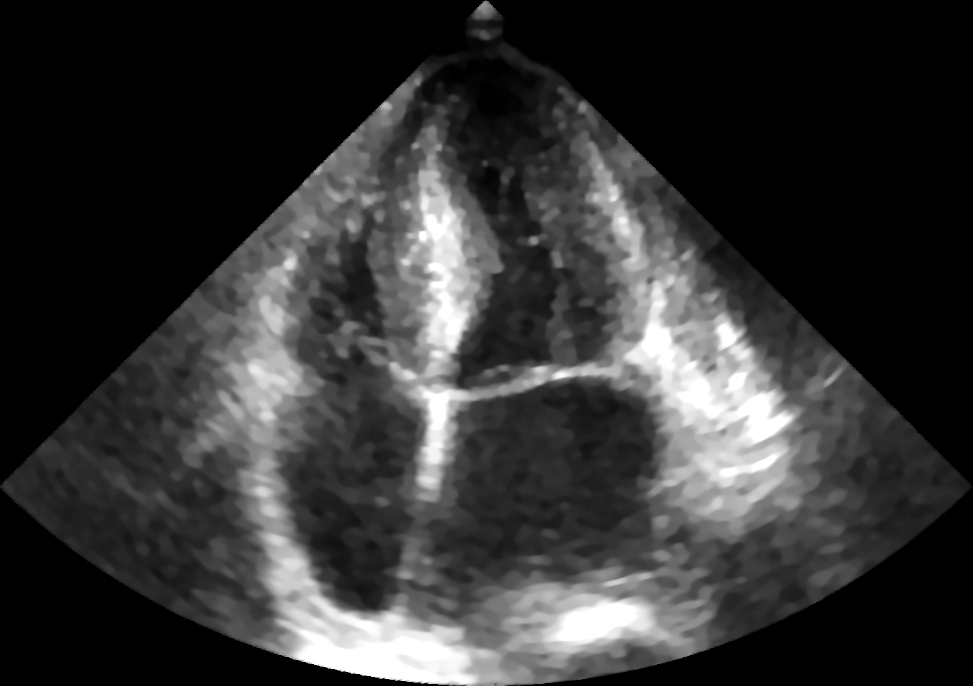
\includegraphics[width=\textwidth]{figures/cardiac3_osrad.png}};
      \spy on (0.1, 0.2) in node [redwindow, anchor=north] at ($(figA.south)$);
    \end{tikzpicture}
    \caption{OSRAD}
  \end{subfigure}%
  \begin{subfigure}[b]{0.15\textwidth}
    \begin{tikzpicture}[
        spy using outlines={%
          rectangle, magnification=3,size=\textwidth,
          every spy on node/.append style={transparentwindow}
        }
      ]
      \node (figA) at (0.0,0.0) {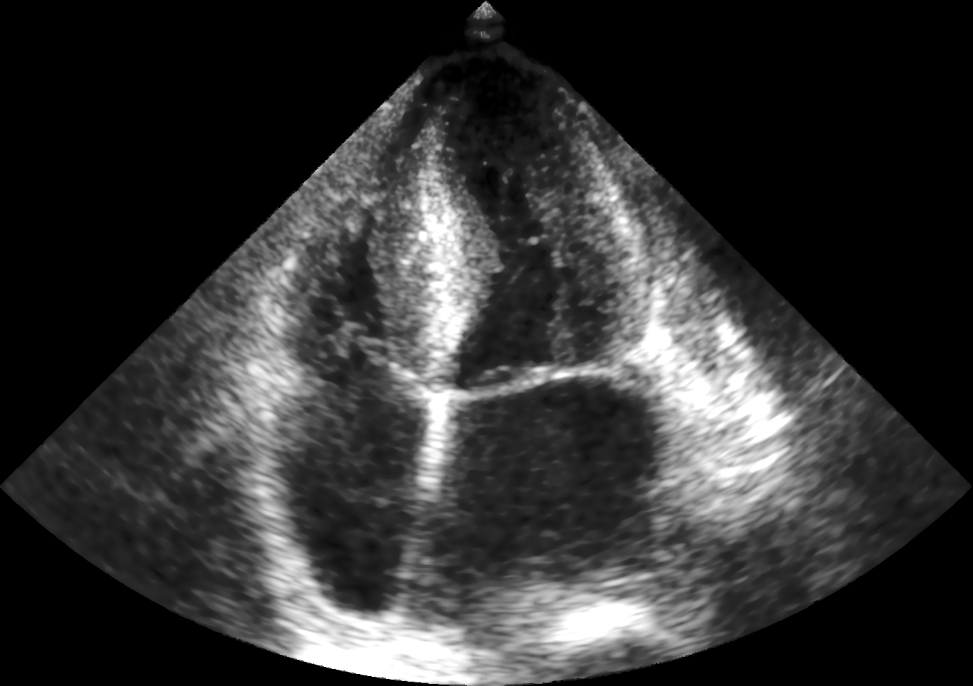
\includegraphics[width=\textwidth]{figures/cardiac3_admss.png}};
      \spy on (0.1, 0.2) in node [redwindow, anchor=north] at ($(figA.south)$);
    \end{tikzpicture}
    \caption{ADMSS}
  \end{subfigure}%
  \begin{subfigure}[b]{0.15\textwidth}
    \begin{tikzpicture}[
        spy using outlines={%
          rectangle, magnification=3,size=\textwidth,
          every spy on node/.append style={transparentwindow}
        }
      ]
      \node (figA) at (0.0,0.0) {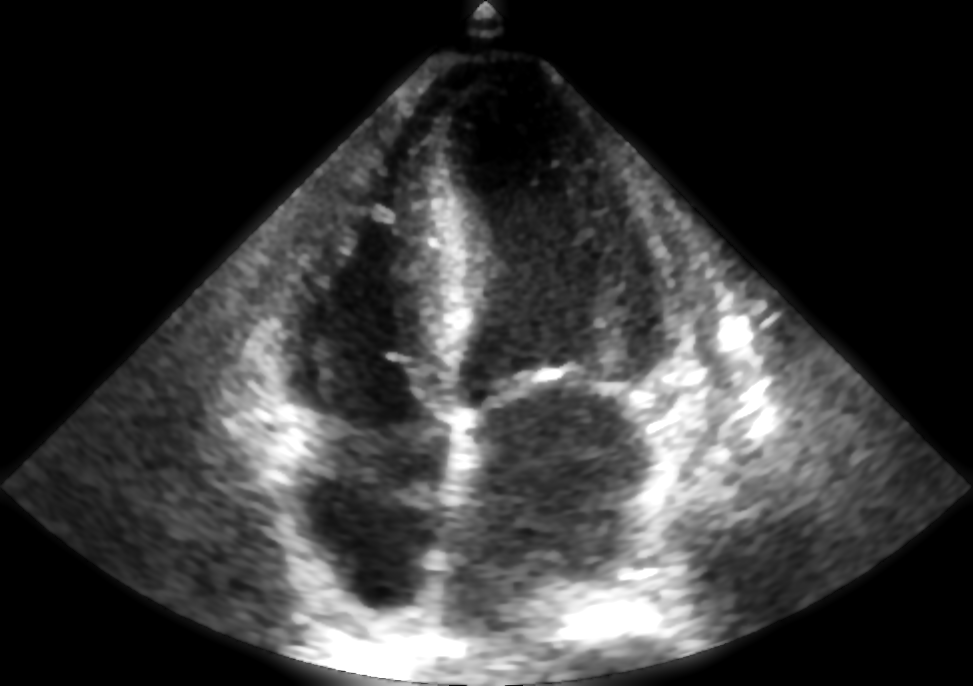
\includegraphics[width=\textwidth]{figures/cardiac3_lpndsf.png}};
      \spy on (0.1, 0.2) in node [redwindow, anchor=north] at ($(figA.south)$);
    \end{tikzpicture}
    \caption{LPNDSF}
  \end{subfigure}%
  \begin{subfigure}[b]{0.15\textwidth}
    \begin{tikzpicture}[
        spy using outlines={%
          rectangle,magnification=3,size=\textwidth,
          every spy on node/.append style={transparentwindow}
        }
      ]
      \node (figA) at (0.0,0.0) {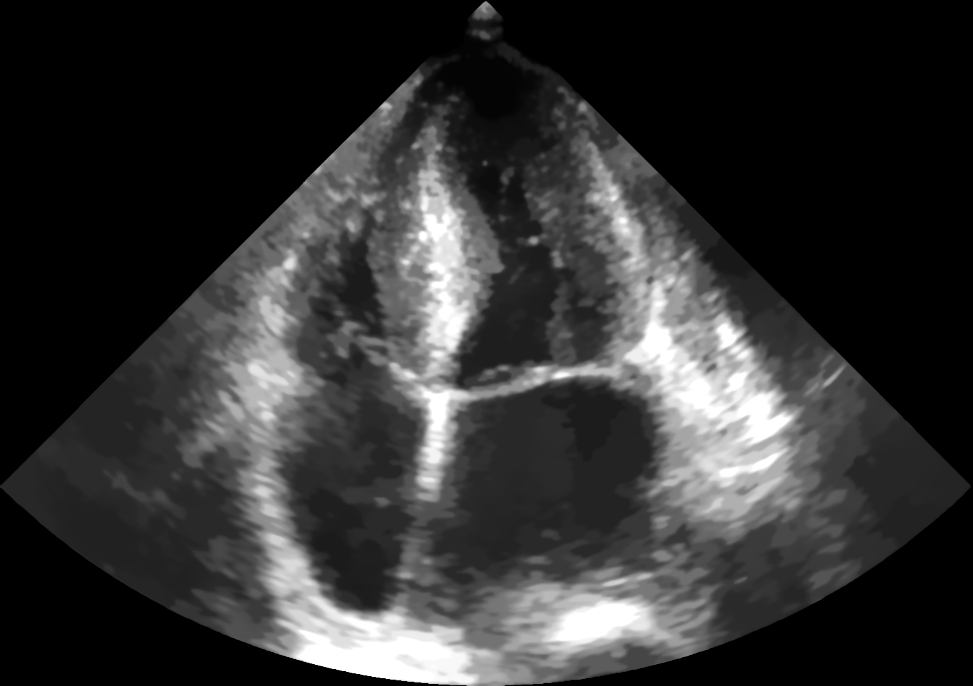
\includegraphics[width=\textwidth]{figures/cardiac3_mnlm.png}};
      \spy on (0.1, 0.2) in node [redwindow, anchor=north] at ($(figA.south)$);
    \end{tikzpicture}
    \caption{MNLM}
  \end{subfigure}%
  \begin{subfigure}[b]{0.15\textwidth}
    \begin{tikzpicture}[
        spy using outlines={%
          rectangle,magnification=3,size=\textwidth,
          every spy on node/.append style={transparentwindow}
        }
      ]
      \node (figA) at (0.0,0.0) {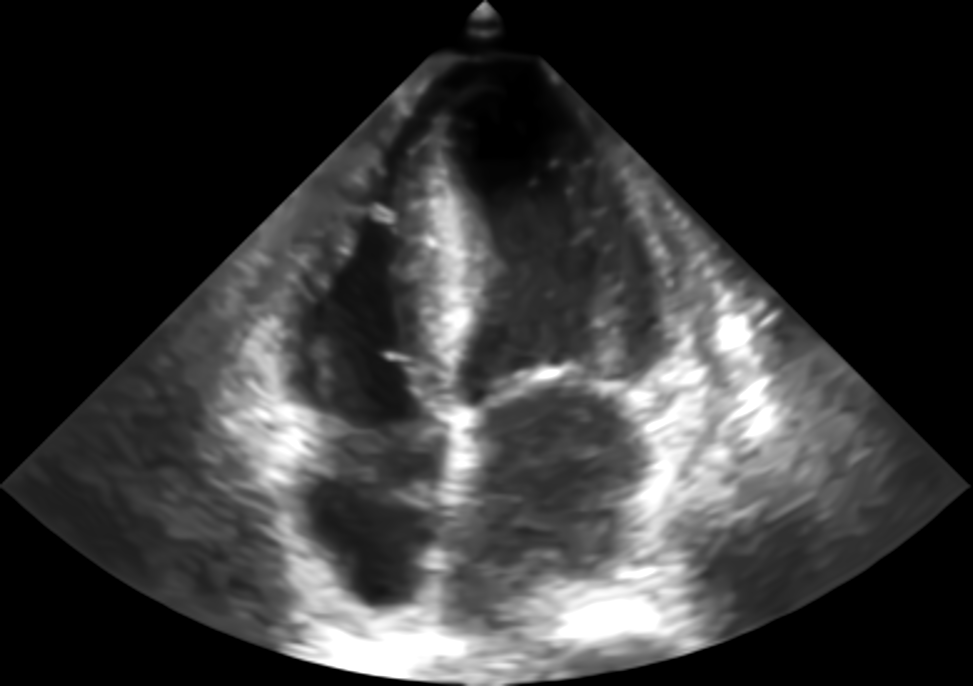
\includegraphics[width=\textwidth]{figures/cardiac3_nllr.png}};
      \spy on (0.1, 0.2) in node [redwindow, anchor=north] at ($(figA.south)$);
    \end{tikzpicture}
    \caption{NLLR}
  \end{subfigure}%
  \begin{subfigure}[b]{0.15\textwidth}
    \begin{tikzpicture}[
        spy using outlines={%
          rectangle,magnification=3,size=\textwidth,
          every spy on node/.append style={transparentwindow}
        }
      ]
      \node (figA) at (0.0,0.0) {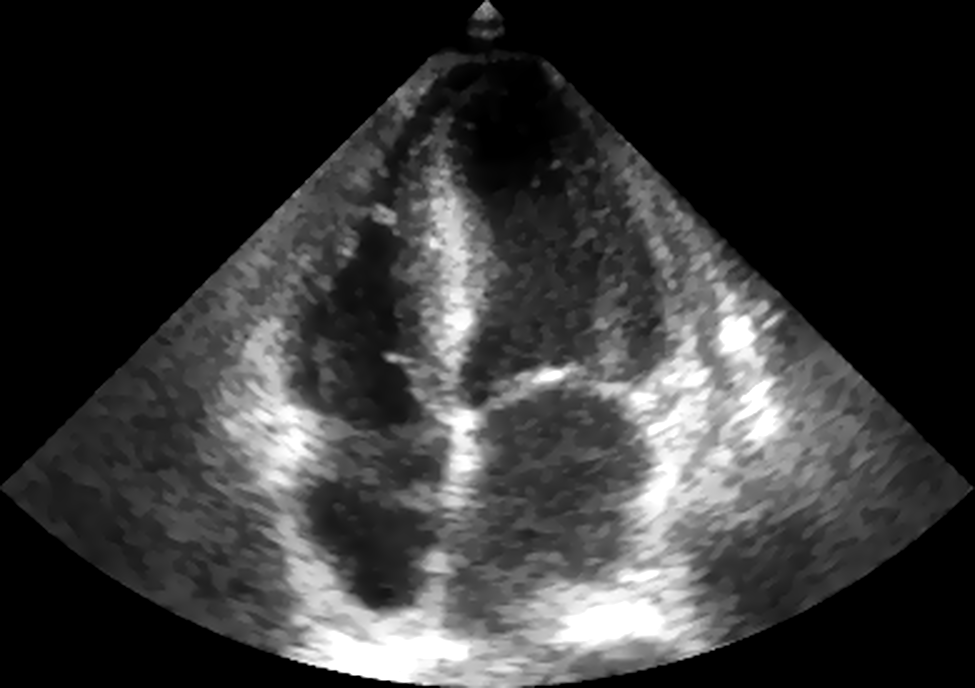
\includegraphics[width=\textwidth]{figures/cardiac3_pfdtv.png}};
      \spy on (0.1, 0.2) in node [redwindow, anchor=north] at ($(figA.south)$);
    \end{tikzpicture}
    \caption{PFDTV}
  \end{subfigure}\\
  %% \begin{subfigure}[b]{0.15\textwidth}
  %%   \begin{tikzpicture}[
  %%       spy using outlines={%
  %%         rectangle,magnification=3,size=\textwidth,
  %%         every spy on node/.append style={transparentwindow}
  %%       }
  %%     ]
  %%     \node (figA) at (0.0,0.0) {\includegraphics[width=\textwidth, trim={4cm 4cm 4cm 0cm}, clip]{figures/cardiac3_clpdQ.png}};
  %%     \spy on (0.1, 0.2) in node [redwindow, anchor=north] at ($(figA.south)$);
  %%   \end{tikzpicture}
  %%   \caption{CLPD-SSNR}
  %% \end{subfigure}%
  \begin{subfigure}[b]{0.15\textwidth}
    \begin{tikzpicture}[
        spy using outlines={%
          rectangle,magnification=3,size=\textwidth,
          every spy on node/.append style={transparentwindow}
        }
      ]
      \node (figA) at (0.0,0.0) {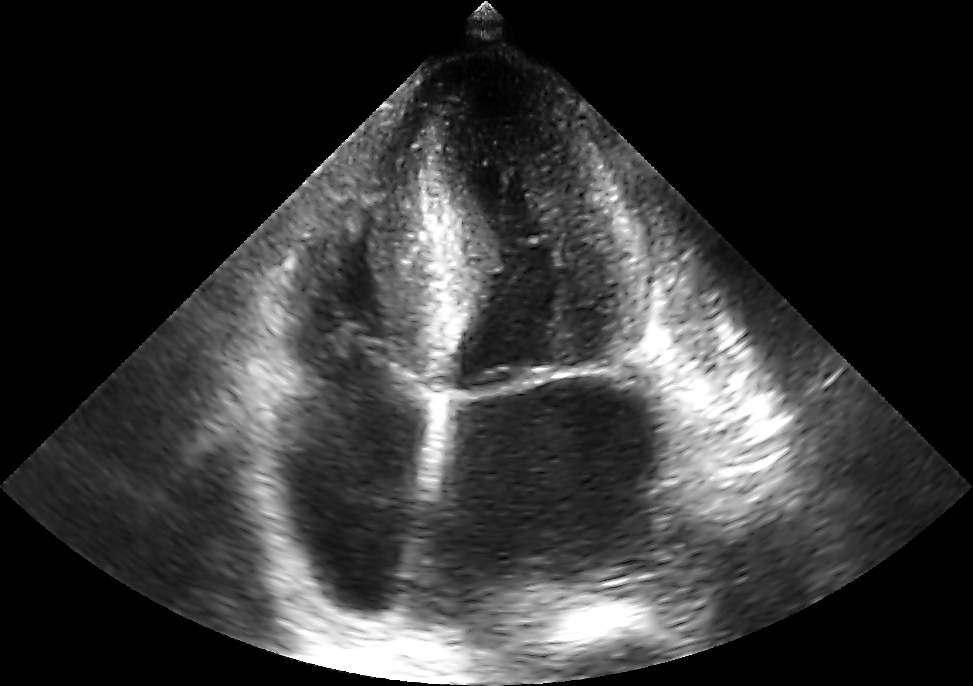
\includegraphics[width=\textwidth]{figures/cardiac3_clpda.png}};
      \spy on (0.1, 0.2) in node [redwindow, anchor=north] at ($(figA.south)$);
    \end{tikzpicture}
    \caption{CLPD-A}
  \end{subfigure}%
  \begin{subfigure}[b]{0.15\textwidth}
    \begin{tikzpicture}[
        spy using outlines={%
          rectangle,magnification=3,size=\textwidth,
          every spy on node/.append style={transparentwindow}
        }
      ]
      \node (figA) at (0.0,0.0) {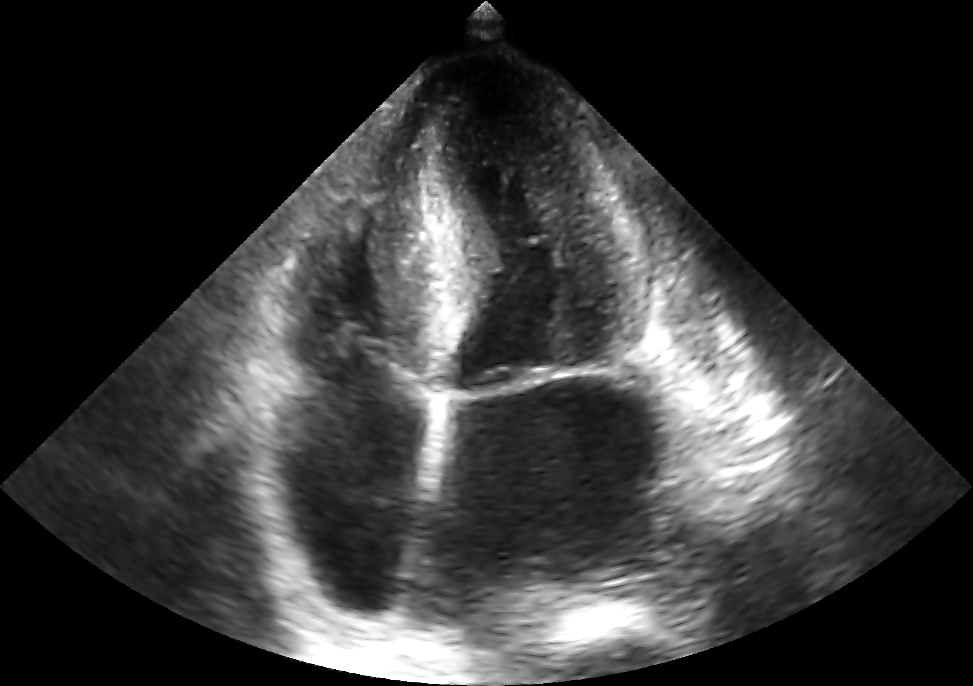
\includegraphics[width=\textwidth]{figures/cardiac3_clpdb.png}};
      \spy on (0.1, 0.2) in node [redwindow, anchor=north] at ($(figA.south)$);
    \end{tikzpicture}
    \caption{CLPD-B}
  \end{subfigure}%
  \begin{subfigure}[b]{0.15\textwidth}
    \begin{tikzpicture}[
        spy using outlines={%
          rectangle,magnification=3,size=\textwidth,
          every spy on node/.append style={transparentwindow}
        }
      ]
      \node (figA) at (0.0,0.0) {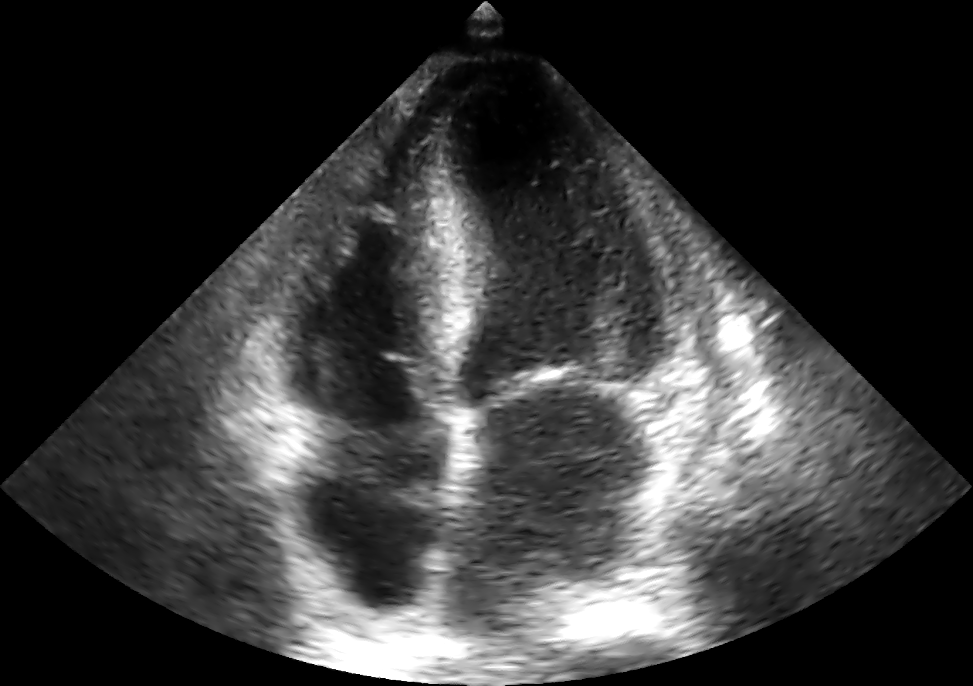
\includegraphics[width=\textwidth]{figures/cardiac3_clpde.png}};
      \spy on (0.1, 0.2) in node [redwindow, anchor=north] at ($(figA.south)$);
    \end{tikzpicture}
    \caption{CLPD-E}
  \end{subfigure}%
  \begin{subfigure}[b]{0.15\textwidth}
    \begin{tikzpicture}[
        spy using outlines={%
          rectangle,magnification=3,size=\textwidth,
          every spy on node/.append style={transparentwindow}
        }
      ]
      \node (figA) at (0.0,0.0) {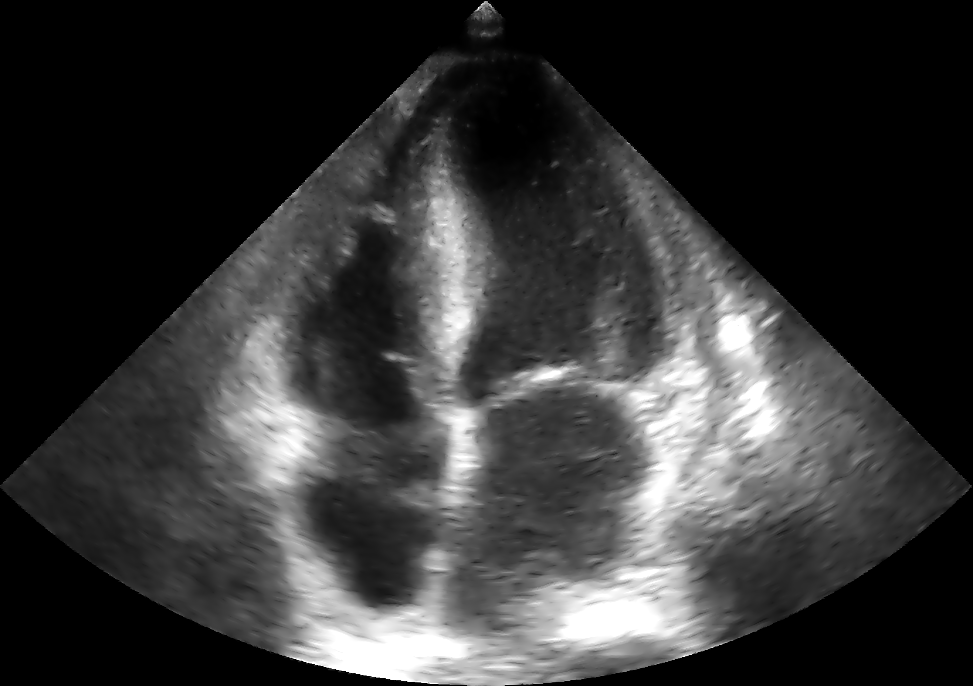
\includegraphics[width=\textwidth]{figures/cardiac3_clpdf.png}};
      \spy on (0.1, 0.2) in node [redwindow, anchor=north] at ($(figA.south)$);
    \end{tikzpicture}
    \caption{CLPD-F}
  \end{subfigure}%
  \begin{subfigure}[b]{0.15\textwidth}
    \begin{tikzpicture}[
        spy using outlines={%
          rectangle,magnification=3,size=\textwidth,
          every spy on node/.append style={redwindow}
        }
      ]
      \node (figA) at (0.0,0.0) {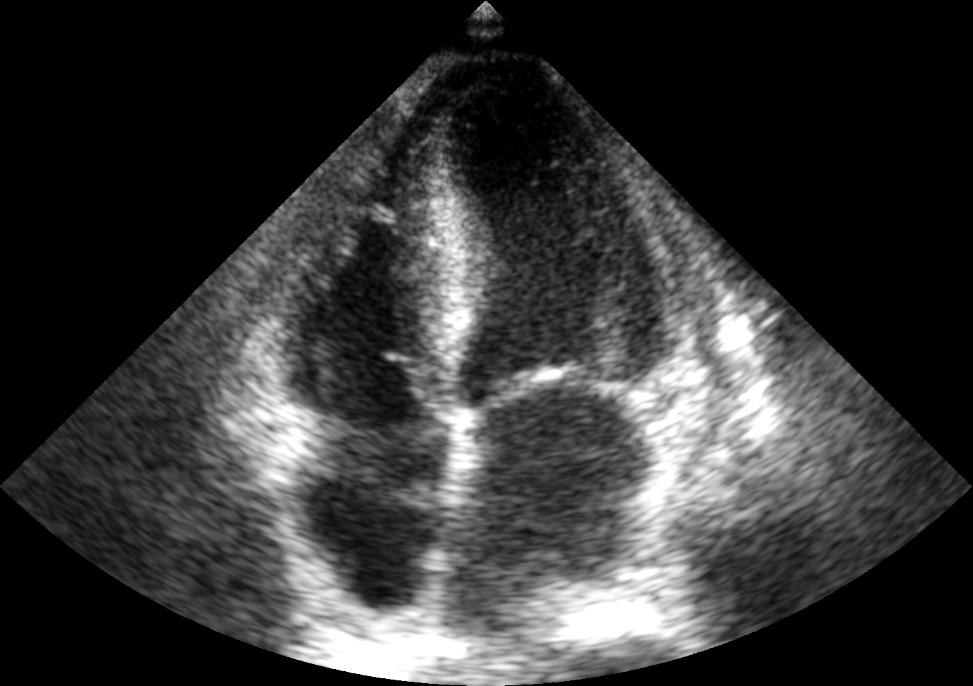
\includegraphics[width=\textwidth]{figures/cardiac3.png}};
      \spy on (0.1, 0.2) in node [redwindow, anchor=north] at ($(figA.south)$);
    \end{tikzpicture}
    \caption{Original}\label{fig:cardiac3_original}
  \end{subfigure}
  \caption{
    Results on echocardiographic 4-chamber view.
    The red squares are zooming on the left-ventricle.
  }\label{fig:cardiac3}
  \vspace{-0.15in}
\end{figure*}


\subsubsection{Quantitative Results}
The quantatitive results using objective performance metrics are shown in~\cref{table:liver1}.
First, we can see that the SSNR values obtained using the CLPDs are worse compared to the baselines except for CLPD-obj., which is natural since it was explicitly tuned to obtain a high SSNR.
This shows that, while it is definitely possible to obtain a high SSNR with the CLPD, none of the sonographers preferred a high SSNR.
Instead, they preferred to preserve some level of speckle noise.
In contrast, all of the baselines except for ADMSS obtained higher SSNR.
In particular, the MNLM obtains the highest leverl of SSNR, which supports the statement that non-local means methods are excellent at removing speckle (which is unfortunately, not desirable).

Meanwhile, when looking at other metrics than the SSNR, the results look quite different.
The CLPDs obtained both high SSIM and high \(S_3\) overall.
Only ADMSS obtained a high SSIM, which is natural since it refrains diffusing tissues.
CLPDs on the other hand all resulted in high levels of SSIMs, which shows that sonographers strongly prefer images that do not look different from the original image.

Lastly, when looking at the \(S_3\) metric, we can see that all CLPDs obtained much higher values.
This shows that the CLPD is capable of conserving sharpness, and that sonographers strongly prefer sharp-looking images.
In fact, many of the participating sonographers explicitly stated that they ``do not want to trade sharpness for less speckle''.
Our results clearly reflect this sentiment.
For this reason, while the NLLR is very good at reinforcing strucutres and reducing speckle, it results in images that are significantly blurry both qualititatively and quantitatively (according to \(S_3\)), which limits its clinical value.


\subsection{Experiment with Echocardocraphic 4-Chamber View}
We present results on echocardiographic images.
We first present experiments performed on a 4-chamber image shown in~\cref{fig:cardiac3_original}.

\subsubsection{Quanlitative Results}

\begin{table}
  \centering
  \caption{Objective Performance Comparison on a Liver}
  \begin{threeparttable}
  \begin{tabular}{llrrrrr}
    \toprule
    & \multicolumn{1}{c}{\textbf{Algorithm}}
    & \multicolumn{1}{c}{\textbf{gCNR}}
    & \multicolumn{1}{c}{\textbf{CNR}}
    & \multicolumn{1}{c}{\textbf{SNR}}
    & \multicolumn{1}{c}{\textbf{SSIM}}
    & \multicolumn{1}{c}{\(\mathbf{S_{3}}\)}\\
    & \multicolumn{1}{c}{}
    & \multicolumn{1}{c}{}
    & \texttt{[dB]}
    & \texttt{[dB]}
    & \multicolumn{1}{c}{}
    & \multicolumn{1}{c}{} \\\midrule
    \multirow{6}{*}{Baselines}
    & OSRAD  & 0.490          & -1.62          & 4.51          & 0.891          & 0.500 \\
    & ADMSS  & 0.467          & -1.67          & 4.33          & \textbf{0.967} & 0.204 \\
    & LPNDSF & 0.473          & -1.67          & 4.39          & 0.868          & 0.458 \\
    & MNLM   & \textbf{0.534} & \textbf{-1.61} & 4.42          & 0.918          & 0.414 \\
    & NLLR   & \textbf{0.501} & \textbf{-1.60} & 4.61          & 0.857          & 0.042\\
    & PFDTV  & 0.480          & -1.65          & 4.49          & 0.865          & 0.155 \\\midrule
    \multirow{4}{*}{This work}
    & CLPD-A & 0.484          & -1.64          & \textbf{4.64} & \textbf{0.957} & \textbf{0.858} \\
    & CLPD-B & \textbf{0.496} & \textbf{-1.55} & \textbf{4.69} & \textbf{0.949} & \textbf{0.685} \\
    & CLPD-E & 0.476          & -1.63          & \textbf{4.61} & \textbf{0.961} & \textbf{0.507} \\
    & CLPD-F & \textbf{0.507} & \textbf{-1.50} & \textbf{4.79} & 0.920          & \textbf{0.705} \\\bottomrule
  \end{tabular}
  \begin{tablenotes}
    \item[*] The performance of the top 4 algorithms for each metric are shown in bold face.
  \end{tablenotes}
  \end{threeparttable}
\end{table}
%
\paragraph{Quantitative Results}

\subsection{Experiment with Echocardocraphic Parasternal Long-Axis View}



\begin{figure*}
  \vspace{-0.1in}
  \centering
  \begin{subfigure}[b]{0.15\textwidth}
    \begin{tikzpicture}[
        spy using outlines={%
          rectangle,magnification=3,size=\textwidth,
          every spy on node/.append style={transparentwindow}
        }
      ]
      \node (figA) at (0.0,0.0) {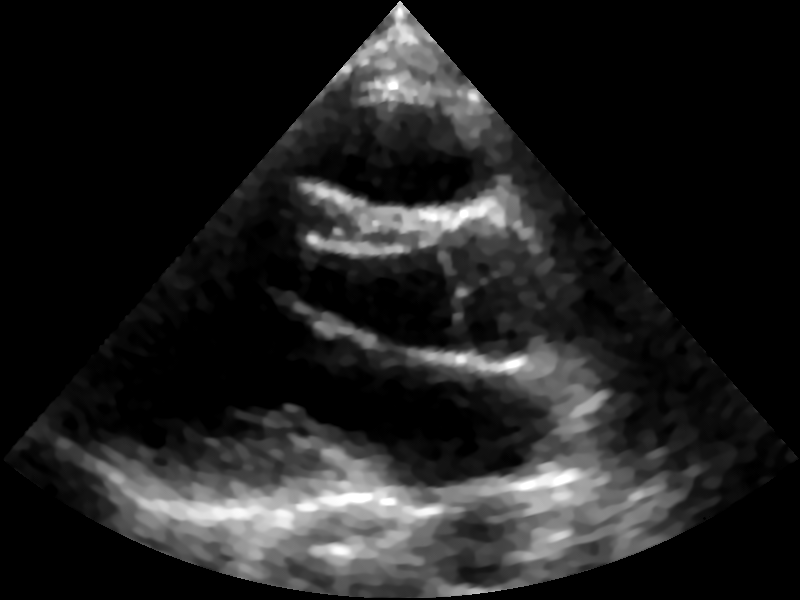
\includegraphics[width=\textwidth]{figures/cardiac1_osrad.png}};
      \spy on (0.05, 0.05) in node [redwindow, anchor=north] at ($(figA.south)$);
    \end{tikzpicture}
    \caption{OSRAD}
  \end{subfigure}%
  \begin{subfigure}[b]{0.15\textwidth}
    \begin{tikzpicture}[
        spy using outlines={%
          rectangle, magnification=3,size=\textwidth,
          every spy on node/.append style={transparentwindow}
        }
      ]
      \node (figA) at (0.0,0.0) {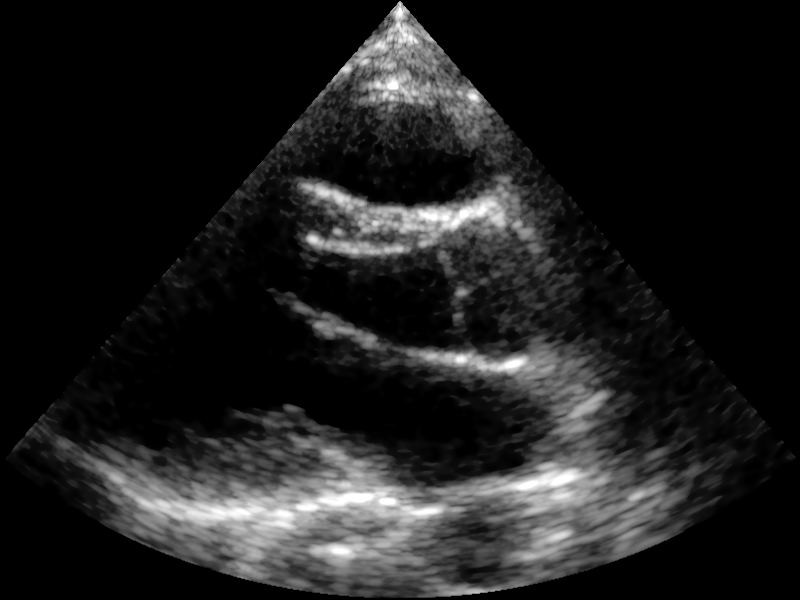
\includegraphics[width=\textwidth]{figures/cardiac1_admss.png}};
      \spy on (0.05, 0.05) in node [redwindow, anchor=north] at ($(figA.south)$);
    \end{tikzpicture}
    \caption{ADMSS}
  \end{subfigure}%
  \begin{subfigure}[b]{0.15\textwidth}
    \begin{tikzpicture}[
        spy using outlines={%
          rectangle, magnification=3,size=\textwidth,
          every spy on node/.append style={transparentwindow}
        }
      ]
      \node (figA) at (0.0,0.0) {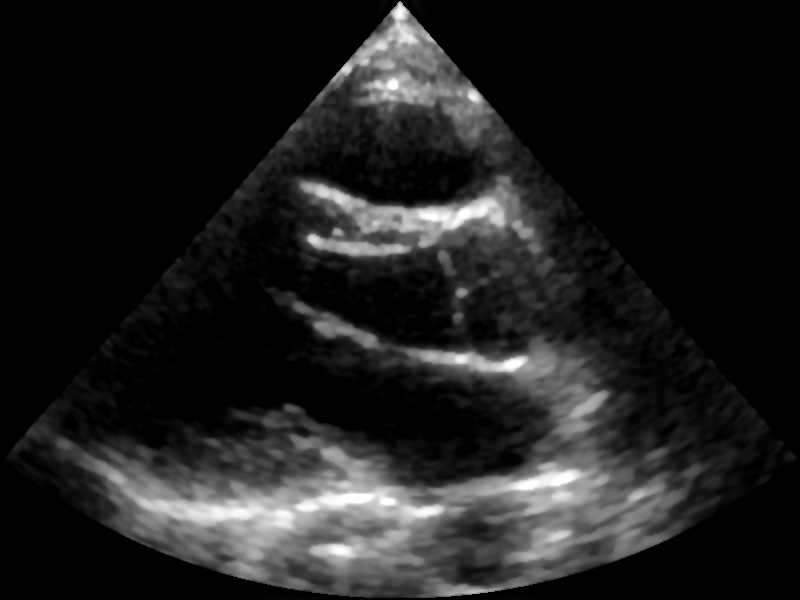
\includegraphics[width=\textwidth]{figures/cardiac1_lpndsf.png}};
      \spy on (0.05, 0.05) in node [redwindow, anchor=north] at ($(figA.south)$);
    \end{tikzpicture}
    \caption{LPNDSF}
  \end{subfigure}%
  \begin{subfigure}[b]{0.15\textwidth}
    \begin{tikzpicture}[
        spy using outlines={%
          rectangle,magnification=3,size=\textwidth,
          every spy on node/.append style={transparentwindow}
        }
      ]
      \node (figA) at (0.0,0.0) {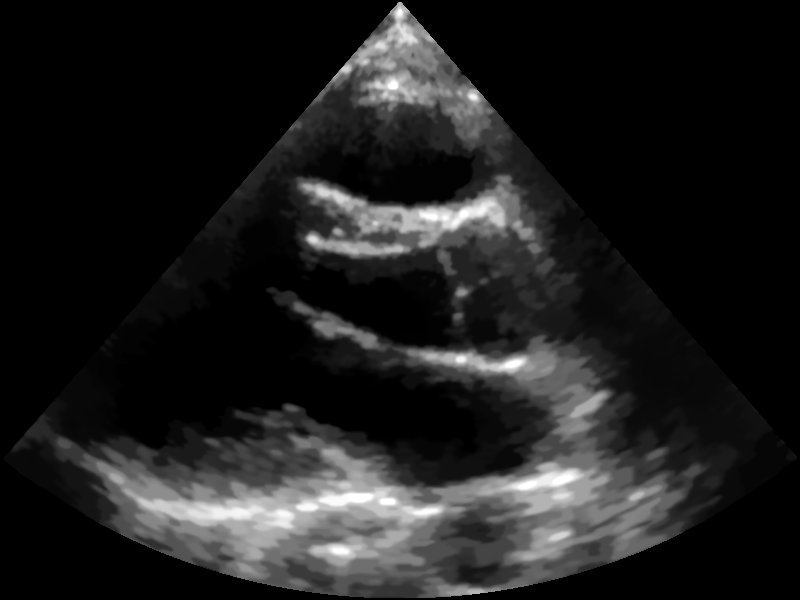
\includegraphics[width=\textwidth]{figures/cardiac1_mnlm.png}};
      \spy on (0.05, 0.05) in node [redwindow, anchor=north] at ($(figA.south)$);
    \end{tikzpicture}
    \caption{MNLM}
  \end{subfigure}%
  \begin{subfigure}[b]{0.15\textwidth}
    \begin{tikzpicture}[
        spy using outlines={%
          rectangle,magnification=3,size=\textwidth,
          every spy on node/.append style={transparentwindow}
        }
      ]
      \node (figA) at (0.0,0.0) {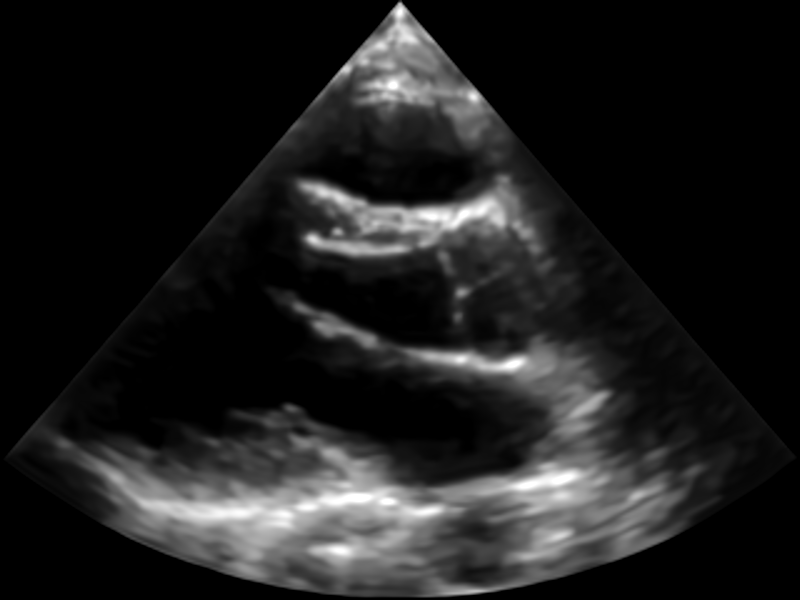
\includegraphics[width=\textwidth]{figures/cardiac1_nllr.png}};
      \spy on (0.05, 0.05) in node [redwindow, anchor=north] at ($(figA.south)$);
    \end{tikzpicture}
    \caption{NLLR}
  \end{subfigure}%
  \begin{subfigure}[b]{0.15\textwidth}
    \begin{tikzpicture}[
        spy using outlines={%
          rectangle,magnification=3,size=\textwidth,
          every spy on node/.append style={transparentwindow}
        }
      ]
      \node (figA) at (0.0,0.0) {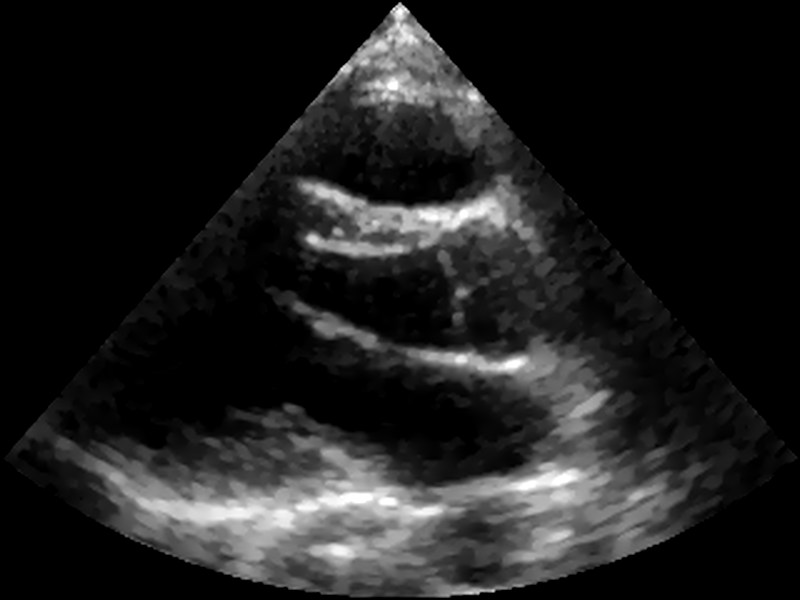
\includegraphics[width=\textwidth]{figures/cardiac1_pfdtv.png}};
      \spy on (0.05, 0.05) in node [redwindow, anchor=north] at ($(figA.south)$);
    \end{tikzpicture}
    \caption{PFDTV}
  \end{subfigure}\\
  %% \begin{subfigure}[b]{0.15\textwidth}
  %%   \begin{tikzpicture}[
  %%       spy using outlines={%
  %%         rectangle,magnification=3,size=\textwidth,
  %%         every spy on node/.append style={transparentwindow}
  %%       }
  %%     ]
  %%     \node (figA) at (0.0,0.0) {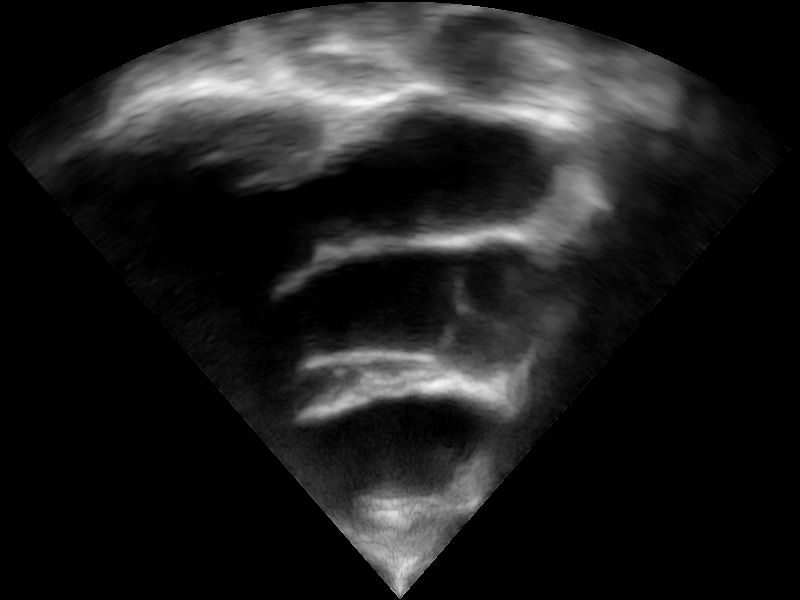
\includegraphics[width=\textwidth, trim={4cm 4cm 4cm 0cm}, clip]{figures/cardiac1_clpdQ.png}};
  %%     \spy on (0.05, 0.05) in node [redwindow, anchor=north] at ($(figA.south)$);
  %%   \end{tikzpicture}
  %%   \caption{CLPD-SSNR}
  %% \end{subfigure}%
  \begin{subfigure}[b]{0.15\textwidth}
    \begin{tikzpicture}[
        spy using outlines={%
          rectangle,magnification=3,size=\textwidth,
          every spy on node/.append style={transparentwindow}
        }
      ]
      \node (figA) at (0.0,0.0) {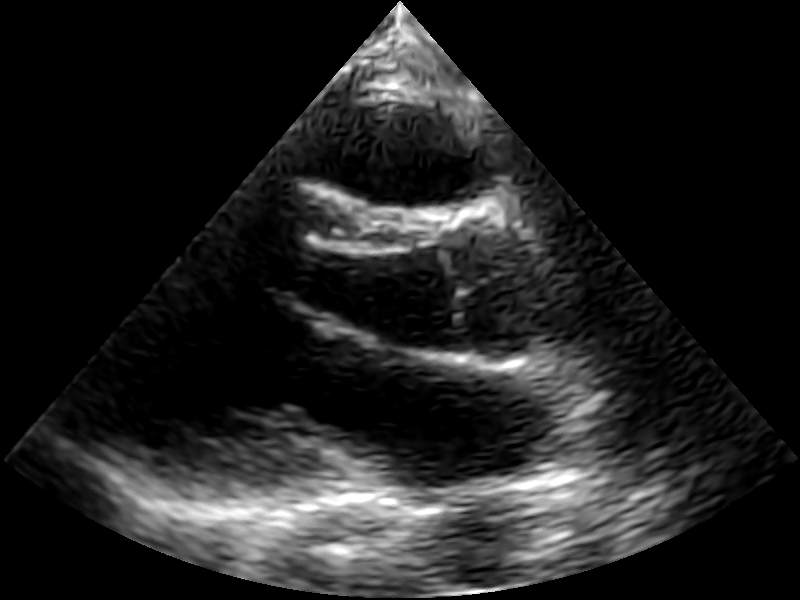
\includegraphics[width=\textwidth]{figures/cardiac1_clpda.png}};
      \spy on (0.05, 0.05) in node [redwindow, anchor=north] at ($(figA.south)$);
    \end{tikzpicture}
    \caption{CLPD-A}
  \end{subfigure}%
  \begin{subfigure}[b]{0.15\textwidth}
    \begin{tikzpicture}[
        spy using outlines={%
          rectangle,magnification=3,size=\textwidth,
          every spy on node/.append style={transparentwindow}
        }
      ]
      \node (figA) at (0.0,0.0) {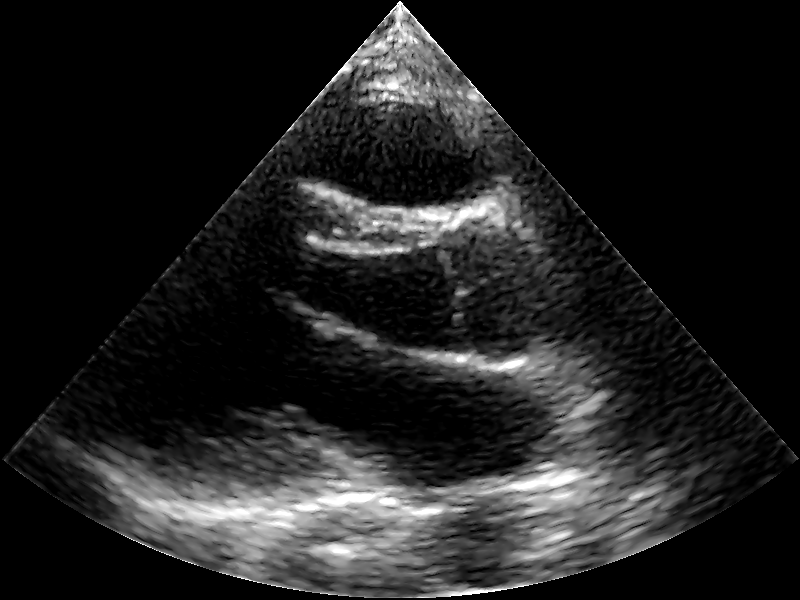
\includegraphics[width=\textwidth]{figures/cardiac1_clpdb.png}};
      \spy on (0.05, 0.05) in node [redwindow, anchor=north] at ($(figA.south)$);
    \end{tikzpicture}
    \caption{CLPD-B}
  \end{subfigure}%
  \begin{subfigure}[b]{0.15\textwidth}
    \begin{tikzpicture}[
        spy using outlines={%
          rectangle,magnification=3,size=\textwidth,
          every spy on node/.append style={transparentwindow}
        }
      ]
      \node (figA) at (0.0,0.0) {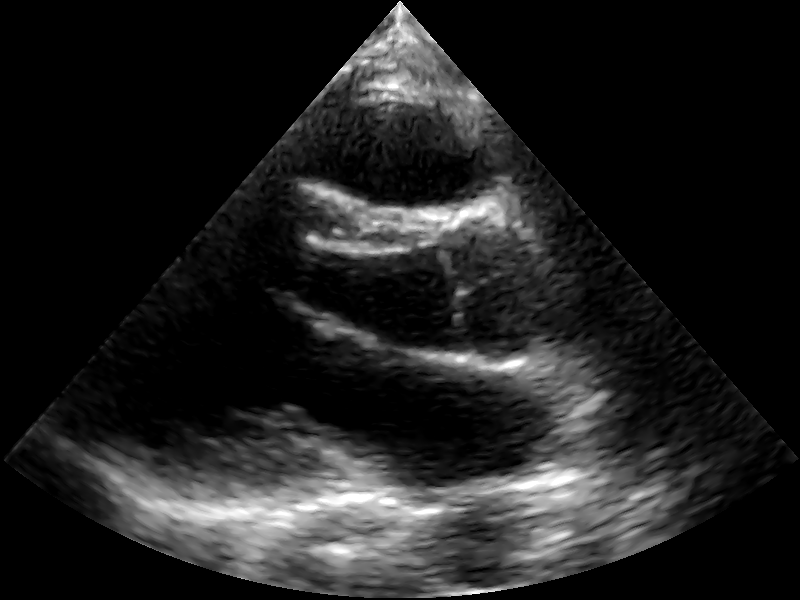
\includegraphics[width=\textwidth]{figures/cardiac1_clpdc.png}};
      \spy on (0.05, 0.05) in node [redwindow, anchor=north] at ($(figA.south)$);
    \end{tikzpicture}
    \caption{CLPD-C}
  \end{subfigure}%
  \begin{subfigure}[b]{0.15\textwidth}
    \begin{tikzpicture}[
        spy using outlines={%
          rectangle,magnification=3,size=\textwidth,
          every spy on node/.append style={transparentwindow}
        }
      ]
      \node (figA) at (0.0,0.0) {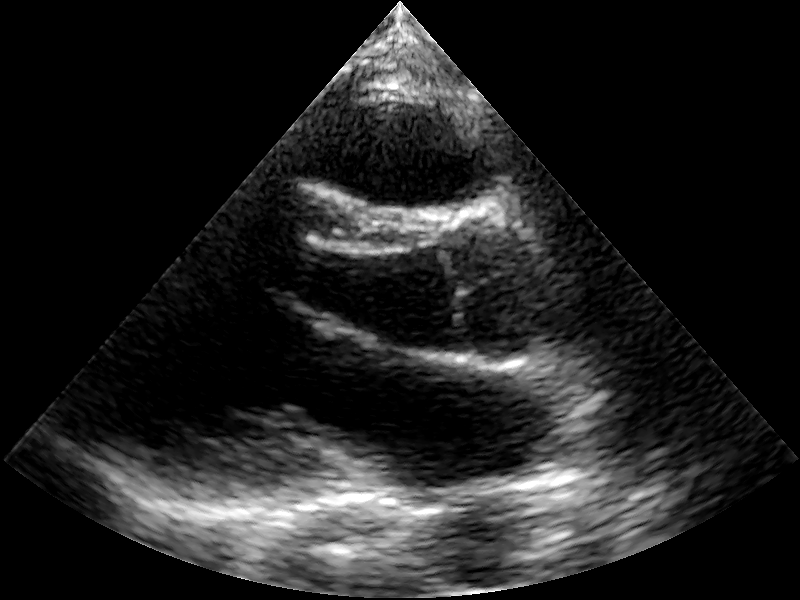
\includegraphics[width=\textwidth]{figures/cardiac1_clpdd.png}};
      \spy on (0.05, 0.05) in node [redwindow, anchor=north] at ($(figA.south)$);
    \end{tikzpicture}
    \caption{CLPD-D}
  \end{subfigure}%
  \begin{subfigure}[b]{0.15\textwidth}
    \begin{tikzpicture}[
        spy using outlines={%
          rectangle,magnification=3,size=\textwidth,
          every spy on node/.append style={redwindow}
        }
      ]
      \node (figA) at (0.0,0.0) {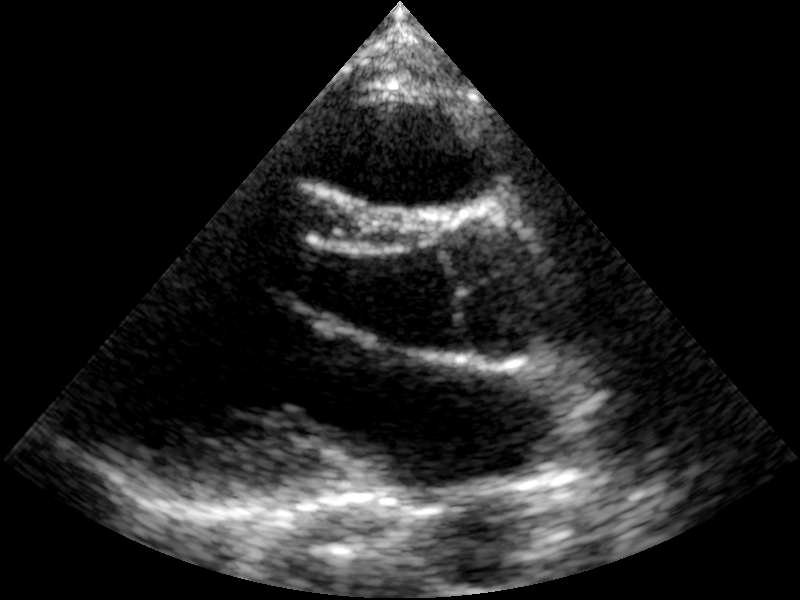
\includegraphics[width=\textwidth]{figures/cardiac1.png}};
      \spy on (0.05, 0.05) in node [redwindow, anchor=north] at ($(figA.south)$);
    \end{tikzpicture}
    \caption{Original}
  \end{subfigure}
  \caption{Results on echocardiography parasternal long-axis view.}\label{fig:cardiac1}
  \vspace{-0.1in}
\end{figure*}

%%% Local Variables:
%%% TeX-master: "master"
%%% End:


%%% Local Variables:
%%% TeX-master: "master"
%%% End:
